
\documentclass[11pt]{article}

% ---------- Packages ----------
\usepackage[margin=1in]{geometry}
\usepackage{amsmath,amssymb,mathtools}
\usepackage{amsthm}
\usepackage{enumitem}
\usepackage{hyperref}
\usepackage{tikz}
\usetikzlibrary{arrows.meta,calc,positioning,decorations.markings}
\newtheorem{theorem}{Theorem}[section]

\newtheorem{metalemma}[theorem]{Meta Lemma}
\newtheorem{proposition}[theorem]{Proposition}
\newtheorem{corollary}[theorem]{Corollary}
\newtheorem{problem}[theorem]{Problem}

\newtheorem*{theorem**}{Theorem\theoremnum}
\newenvironment{theorem*}[1][]{%
  % https://tex.stackexchange.com/a/53091/5764
  \edef\theoremnum{\if\relax\detokenize{#1}\relax\else~#1\fi}% Store theorem number
  \begin{theorem**}
}{%
  \end{theorem**}
}  

%definitions}
\theoremstyle{definition}
\newtheorem{definition}[theorem]{Definition}
\newtheorem{observation}{Observation}

% ---------- Theorem environments ----------
\theoremstyle{plain}
\newtheorem{lemma}[theorem]{Lemma}
\theoremstyle{remark}
\newtheorem{remark}[theorem]{Remark}

% ---------- Macros ----------
\newcommand{\Cay}{\mathrm{Cay}}
\newcommand{\Sch}{\mathrm{Sch}}
\newcommand{\Core}{\mathrm{Core}}
\newcommand{\lab}{\mathrm{lab}}
\newcommand{\Faces}{\mathrm{Faces}}
\newcommand{\End}{\mathrm{End}}

% ---------- TikZ styles ----------
\tikzset{
  vtx/.style={circle,draw,inner sep=1.6pt},
  basevtx/.style={circle,draw,inner sep=1.6pt, double},
  edge/.style={-Latex,thick},
  uedge/.style={thick},
  loop/.style={thick},
  treedge/.style={thick,dashed},
  nonte/.style={thick},
  face/.style={draw,thick},
  every node/.style={font=\small}
}

\title{A Handbook of Graphs and Diagrams in Group Theory and Topology\\
\large Detailed constructions, reconstructions, and TikZ drawings}
\author{Hanwen Shen\\ Stevens Institute of Technology}

\date{December 2025}

\begin{document}
\maketitle
\begin{abstract}
This handbook collects a unified “diagrammatic toolkit” for combinatorial group theory and low-dimensional topology.
Its goal is practical: to make the standard graphs, diagrams, and 2-complexes that encode algebraic statements
easy to construct, compare, and use as algorithmic certificates.
For each object, we give (i) a precise definition in a consistent combinatorial model (words, labeled graphs, finite
2-dimensional CW- and polygonal complexes); (ii) an existence/uniqueness statement clarifying what is canonical
(up to label- and basepoint-preserving isomorphism) and what depends on choices; (iii) \textbf{Algorithm A} (Forward)
turning algebraic input into a graph/diagram/complex; (iv) \textbf{Algorithm B} (Inverse) extracting algebraic data or a
certificate back from the combinatorial object; and (v) worked examples drawn in TikZ, with explicit step-by-step
construction and reconstruction.
\end{abstract}
\tableofcontents

% ============================================================
\section{Introduction}
This handbook collect standard graphs and diagrams used in combinatorial group theory and low-dimensional topology. \textbf{Please read textbook for formal study.}

For each object we include:
\begin{itemize}[leftmargin=2em]
\item a definition;
\item an existence/uniqueness theorem (what is canonical, and what is not);
\item \textbf{Algorithm A (Forward)}: algebra/input $\to$ graph/diagram/complex;
\item \textbf{Algorithm B (Inverse)}: graph/diagram/complex $\to$ algebraic data/certificate;
\item \textbf{worked examples with step-by-step construction and reconstruction, each drawn in TikZ}.
\end{itemize}

\medskip
\noindent\textbf{Important meta-convention.}
When we say ``unique up to isomorphism'' we always mean \emph{label-preserving isomorphism} (and basepoint-preserving if a basepoint is part of the data).

% ============================================================

% ============================================================
\section{Conventions}

\subsection{Words, reductions, and lengths}
Fix a finite alphabet of generators $X=\{x_1,\dots,x_n\}$ and let $X^{\pm 1}=X\cup X^{-1}$.
A \emph{word} is a finite string $w=x_{i_1}^{\varepsilon_1}\cdots x_{i_k}^{\varepsilon_k}$ with $\varepsilon_j\in\{\pm1\}$.
Its \emph{length} is $|w|=k$.

A word is \emph{freely reduced} if it has no adjacent cancellation $xx^{-1}$ or $x^{-1}x$.
\textbf{Convention (terminology):} throughout these notes, \emph{reduced} means \emph{freely reduced}.
We write $\mathrm{red}(w)$ for the freely reduced form of $w$ (obtained by repeatedly cancelling adjacent inverse pairs).

A reduced word $w$ is \emph{cyclically reduced} if every cyclic rotation of $w$ is reduced, equivalently the first letter is not inverse to the last letter.

Let $X=\{a,b\}$ and $X^{\pm1}=\{a^{\pm1},b^{\pm1}\}$.

\paragraph{Words (what is / what is not).}
\begin{itemize}[leftmargin=2em]
\item \textbf{Is a word:} $w=a\,b^{-1}\,a\,a^{-1}\,b$ (a finite string of letters in $X^{\pm1}$).
\item \textbf{Is a word:} $w=(a^{-1})^3\,b\,a^2$ (this is just shorthand for $a^{-1}a^{-1}a^{-1} b a a$).
\item \textbf{Not a word (in this model):} $a^{1/2}b$ (exponents other than $\pm1$ are not letters of $X^{\pm1}$).
\item \textbf{Not a word (as a finite string):} $ababab\cdots$ (an infinite string; words here are finite).
\end{itemize}

\paragraph{Free reduction: reduced vs.\ not reduced.}
Recall: \emph{reduced} means \emph{freely reduced}.

\begin{itemize}[leftmargin=2em]
\item \textbf{Not reduced (has adjacent cancellation):}
\[
w_1 = a\,a^{-1}\,b.
\]
Here $a a^{-1}$ cancels, so $\mathrm{red}(w_1)=b$ and $|w_1|=3$, $|\mathrm{red}(w_1)|=1$.

\item \textbf{Not reduced (multiple cancellations):}
\[
w_2 = a\,b\,b^{-1}\,a^{-1}.
\]
Cancel $b b^{-1}$ to get $a a^{-1}$, so $\mathrm{red}(w_2)=\varepsilon$ (the empty word).

\item \textbf{Reduced (no adjacent inverse pairs):}
\[
w_3 = a\,b\,a^{-1}\,b^{-1}.
\]
No adjacent letters are inverse, hence $\mathrm{red}(w_3)=w_3$.

\item \textbf{Reduced (even though inverse letters appear non-adjacently):}
\[
w_4 = a\,b\,a^{-1}.
\]
This is reduced because the $a$ and $a^{-1}$ are not adjacent, so there is no free cancellation.
\end{itemize}

\paragraph{Cyclic reduction: cyclically reduced vs.\ not cyclically reduced.}
A reduced word is \emph{cyclically reduced} iff its first letter is not the inverse of its last letter.

\begin{itemize}[leftmargin=2em]
\item \textbf{Reduced but not cyclically reduced:}
\[
w_5 = a\,b\,a^{-1}.
\]
It is reduced, but the first letter $a$ is inverse to the last letter $a^{-1}$, so it is \emph{not} cyclically reduced.
Indeed, the cyclic rotation $b\,a^{-1}\,a$ is not reduced (it contains $a^{-1}a$).

\item \textbf{Cyclically reduced:}
\[
w_6 = a\,b\,a^{-1}\,b^{-1}.
\]
This is reduced and the first letter $a$ is not inverse to the last letter $b^{-1}$, hence it is cyclically reduced.

\item \textbf{Cyclically reduced (short words):}
\[
w_7 = a,\qquad w_8=b^{-1}.
\]
Any reduced word of length $1$ is cyclically reduced.

\item \textbf{Not cyclically reduced (after reducing first):}
\[
w_9 = a\,b\,b^{-1}\,a^{-1}.
\]
This word is not reduced. After free reduction, $\mathrm{red}(w_9)=\varepsilon$.
(If you only apply the cyclically reduced definition to \emph{reduced} words, you first reduce and then check.)
\end{itemize}


\subsection{Complexity parameters (what ``input size'' means)}
For algorithmic statements we will use the following standard size parameters:
\begin{itemize}[leftmargin=2em]
\item For words: length $|w|$.
\item For a subgroup input $H=\langle w_1,\dots,w_m\rangle\le F(X)$: total input length
\[
L=\sum_{i=1}^m |w_i| \quad \text{(after free reduction).}
\]
\item For a finite graph $\Gamma$: number of vertices $|V|$, edges $|E|$.
\item For a finite 2-complex/diagram $D$: numbers $(|V|,|E|,|F|)$, and total perimeter
\[
P=\sum_{f\in \Faces(D)} |\partial f|.
\]
\item For a finite presentation $\mathcal P=\langle X\mid R\rangle$: total relator length
\[
\|R\|=\sum_{r\in R} |r|.
\]
\end{itemize}
When groups are infinite, one usually works with \emph{implicit} representations (normal forms, rewriting systems, coset enumeration, etc.);
complexity then depends on the chosen representation. We will state complexities in terms of the combinatorial objects actually built (numbers of vertices/edges/faces) and the lengths of words manipulated.


\subsubsection*{Binary vs.\ unary encoding for integers}
An integer $N\ge 0$ may be provided in:
\begin{itemize}[leftmargin=2em]
\item \textbf{Binary encoding:} input size $\langle N\rangle := \lfloor \log_2(N)\rfloor+1$ bits (for $N\ge 1$; and $\langle 0\rangle:=1$).
\item \textbf{Unary encoding:} input size $\Theta(N)$ symbols (rare in group theory, but sometimes used to model ``pseudopolynomial'' behavior).
\end{itemize}
\subsubsection*{Words and presentations: typical examples}
\begin{itemize}[leftmargin=2em]
\item \textbf{Word problem input:} a word $w\in (X^{\pm1})^*$ with size $|w|$.
\item \textbf{Subgroup membership input:} $H=\langle w_1,\dots,w_m\rangle\le F(X)$ together with a query word $w$.
The total size is typically $L+|w|$, where $L=\sum_i |w_i|$ after free reduction.
\item \textbf{Finite presentation input:} $\mathcal P=\langle X\mid R\rangle$ with size
\[
|X|+\|R\|,\qquad \|R\|:=\sum_{r\in R}|r|
\]
(again with relators freely reduced; one may also include the number of relators $|R|$ separately).
\end{itemize}

\subsubsection*{Numeric labels and weights on graphs/complexes}
Often a graph or 2--complex comes with additional integer data (lengths, weights, exponents, capacities).
\begin{itemize}[leftmargin=2em]
\item \textbf{Edge/vertex weights in binary:} if each edge $e\in E$ has an integer weight $w(e)\in\mathbb Z$ given in binary,
the input size includes
\[
\sum_{e\in E}\langle |w(e)|\rangle
\]
(and similarly for vertex weights).
\item \textbf{Geometric coordinates:} if vertices are given by rational coordinates in $\mathbb Q^d$,
write each coordinate as $p/q$ in lowest terms; the input size includes the total bit-length of all numerators/denominators:
\[
\sum_{\text{coords}} \bigl(\langle |p|\rangle+\langle |q|\rangle\bigr).
\]
\end{itemize}

\subsubsection*{Matrices and linear representations (common in algorithmic group theory)}
\begin{itemize}[leftmargin=2em]
\item \textbf{Matrix group input:} generators $A_1,\dots,A_m\in \mathrm{GL}_d(\mathbb Z)$ (or $\mathrm{GL}_d(\mathbb Q)$).
The input size is
\[
m\cdot d^2 \;+\; \sum_{i=1}^m \sum_{j,k} \langle |(A_i)_{jk}|\rangle
\]
for integer entries (or add numerator/denominator bit-lengths for rational entries).
\item \textbf{Word in matrix generators:} a word of length $n$ in the alphabet $\{A_i^{\pm1}\}$ has size $n$ in the word metric,
but the intermediate matrix entries may grow; complexity bounds must specify whether arithmetic is counted in \emph{bit complexity}.
\end{itemize}

\subsubsection*{Automata and rewriting systems (implicit representations)}
When groups or languages are described implicitly, the ``size'' is the description length of the device.
\begin{itemize}[leftmargin=2em]
\item \textbf{Finite automaton input:} a DFA/NFA with $|Q|$ states over alphabet $\Sigma$.
A standard encoding size is
\[
O\bigl(|Q|\cdot|\Sigma|\bigr)
\]
for the transition table (plus the size of the accept set).
\item \textbf{Rewriting system input:} a finite set of rewrite rules $\ell\to r$.
A natural size parameter is the total rule length
\[
\|\mathcal R\|\;:=\;\sum_{(\ell\to r)\in\mathcal R}\bigl(|\ell|+|r|\bigr).
\]
\item \textbf{Straight-line program (SLP) / compressed word:} a context-free grammar producing a single word.
The input size is the number of productions (and total symbol count), which can be exponentially smaller than the expanded word length.
When inputs may be compressed, one must state whether complexity is measured in terms of SLP size or expanded length.
\end{itemize}

\subsubsection*{Common ``input packages'' (worked-size examples)}
\begin{itemize}[leftmargin=2em]
\item \textbf{Van Kampen diagram input:} a finite planar 2--complex $D$ with labels on directed edges.
Size can be taken as $(|V|,|E|,|F|)$ together with the total perimeter $P=\sum_{f}|\partial f|$.
If labels are words over $X^{\pm1}$, add their total length as well.

\item \textbf{Graph-of-groups / Bass--Serre input:} a finite graph $\Gamma$ plus finitely presented vertex/edge groups and attaching maps.
A practical size measure is $|V(\Gamma)|+|E(\Gamma)|$ plus the presentation sizes of all vertex/edge groups and the word-lengths
of images of edge generators under the attaching maps.

\item \textbf{Surface input:} a triangulated surface given by its face list (triples of vertex indices).
Size is $\Theta(|F|)$ plus the bit-length of indices if vertices are named in binary.
\end{itemize}

\subsubsection*{Bit complexity vs.\ unit-cost arithmetic}
When algorithms involve integer arithmetic (e.g.\ matrix multiplication, coordinate computations),
it is important to specify the cost model:
\begin{itemize}[leftmargin=2em]
\item \textbf{Unit-cost RAM model:} each arithmetic operation on machine words costs $O(1)$ (good for fixed-size integers).
\item \textbf{Bit complexity model:} the cost of arithmetic depends on operand bit-length (required for honest bounds when numbers can grow).
\end{itemize}
Unless stated otherwise, we count \emph{bit complexity} whenever integer sizes may grow during the computation.

\paragraph{Remark.}
The same mathematical object can have very different input sizes depending on representation
(e.g.\ an element given by an explicit word vs.\ an SLP-compressed word, or a subgroup given by a generating set vs.\ a Stallings graph).
Accordingly, complexity statements should always specify the representation and which size parameters are being used.



\subsection{$X$-labeled graphs and path labels}
An \emph{$X$-labeled oriented graph} is a directed graph whose directed edges are labeled by $X^{\pm1}$, with the rule:
reversing an edge inverts its label.
For a directed path $p=e_1\cdots e_k$, define $\lab(p)=\lab(e_1)\cdots\lab(e_k)$.

\textbf{Terminology consistency:} when we say \emph{labeled graph} in these notes, we always mean \emph{$X$-labeled} unless explicitly stated otherwise.

A labeled graph is \emph{folded (deterministic)} if for every vertex $v$ and every label $a\in X^{\pm1}$ there is at most one outgoing edge from $v$ with label $a$.
Equivalently, reading a reduced word from a vertex determines at most one reduced path.

\subsection{CW-complexes and polygonal complexes}
A \emph{CW-complex} is a space built by attaching $k$-cells (copies of open disks) inductively via continuous attaching maps on their boundaries.
In these notes we only use \emph{finite 2-dimensional} CW-complexes (0-, 1-, and 2-cells).\cite{hatcher2002}

A \emph{polygonal complex} is a 2-dimensional CW-complex in which each 2-cell is attached along the boundary cycle of a polygon
(an $n$-gon subdivided into $n$ oriented edges), with attaching maps that send edges to edge-paths.
Thus:
\[
\text{polygonal complex} \subseteq \text{(2-dimensional CW-complex)}.
\]
Presentation complexes and van Kampen diagrams are polygonal complexes.


\subsection*{Examples: CW-complexes and polygonal complexes (simple)}

\paragraph{CW-complexes (finite, low-dimensional examples).}
\begin{itemize}[leftmargin=2em]
\item \textbf{A finite graph.}
Any finite graph $\Gamma$ is a $1$--dimensional CW-complex: vertices are $0$--cells and edges are $1$--cells attached at their endpoints.

\item \textbf{The circle $S^1$.}
One $0$--cell $v$ and one $1$--cell $e$ attached with both endpoints mapped to $v$.

\item \textbf{A disk $D^2$.}
One $0$--cell, one $1$--cell forming the boundary circle, and one $2$--cell attached along that boundary loop.

\item \textbf{The sphere $S^2$.}
One $0$--cell and one $2$--cell attached by the constant map $S^1\to$ (the $0$--cell).
(Equivalently, two $2$--cells glued along their boundary circle.)
\end{itemize}

\paragraph{Polygonal complexes (2D CW-complexes with polygonal faces).}
\begin{itemize}[leftmargin=2em]
\item \textbf{A single polygon.}
Take an $n$--gon and attach its boundary edges in a cycle; this is the simplest polygonal complex with one face.

\item \textbf{The torus $T^2$ from one square.}
One vertex, two edges labeled $a,b$, and one square $2$--cell attached by the boundary word
\[
aba^{-1}b^{-1}.
\]
This is a polygonal complex with one $4$--gonal face.

\item \textbf{A presentation complex (one-relator case).}
For $\mathcal P=\langle X\mid r\rangle$, take a wedge of $|X|$ circles (one for each generator) and attach one $2$--cell along the loop labeled by $r$.
This is a polygonal complex whose single face has perimeter $|r|$.

\item \textbf{A van Kampen diagram.}
A van Kampen diagram is a finite planar polygonal complex (topologically a disk) whose faces are labeled by relators (and inverses),
with a distinguished outer boundary cycle labeling a word equal to $1$ in the group.
\end{itemize}

\paragraph{One simple non-example (CW but not polygonal).}
\begin{itemize}[leftmargin=2em]
\item \textbf{A non-combinatorial attachment.}
Attach a $2$--cell to a graph by a continuous map $S^1\to \Gamma$ that is not a combinatorial edge-loop
(e.g.\ it collapses an arc of $S^1$ to a point).
The result is still a $2$--dimensional CW-complex, but it is not polygonal under the combinatorial definition above.
\end{itemize}

\subsection*{What is \emph{not} a CW-complex? (standard non-examples)}

\paragraph{(1) Failure of closure-finiteness: the infinite wedge (Hawaiian earring type).}
Let $H\subset \mathbb{R}^2$ be the \emph{Hawaiian earring}, the union of circles
\[
H=\bigcup_{n\ge 1} C_n,\qquad
C_n=\{(x,y): (x-1/n)^2+y^2=(1/n)^2\},
\]
all tangent at the origin.
This space is \emph{not} a CW-complex: any cell decomposition would force the point of tangency to lie in the closure
of infinitely many $1$--cells, violating the closure-finite condition.

\paragraph{(2) Failure of weak topology: spaces with a ``bad'' quotient topology.}
There are classical examples of cell-like decompositions or quotient spaces where the resulting topology is not the weak topology
coming from cells. Such spaces can be built by gluing disks in a purely set-theoretic way, but the topology is too coarse/fine
to satisfy axiom (W), hence the space is not CW.
(Concrete examples can be found in standard topology texts under ``weak topology fails for CW''.)

\paragraph{(3) Non-Hausdorff spaces (CW-complexes are Hausdorff).}
Every CW-complex is Hausdorff.
Hence any non-Hausdorff space is automatically \emph{not} a CW-complex.
For example, the \emph{line with two origins} is not Hausdorff, so it is not a CW-complex.

\paragraph{(4) The long line (not a CW-complex).}
The (closed) long line is a connected $1$--manifold that is not second countable and has pathological compactness properties.
It is not homotopy equivalent to any CW-complex and, in particular, is not a CW-complex.

\paragraph{Remark.}
Most ``reasonable'' spaces encountered in algebraic topology (manifolds, polyhedra, simplicial complexes, finite graphs,
finite 2--complexes, etc.) are CW-complexes. Non-examples typically arise from infinite accumulation phenomena
(e.g.\ infinitely many cells piling up at a point) or from pathological topologies.

\subsection{Simply connected (precise meaning)}
A space $Y$ is \emph{simply connected} if it is path-connected and every loop $\gamma:S^1\to Y$ is null-homotopic.
Equivalently, $\pi_1(Y)$ is trivial.
For a finite 2-complex/diagram, ``simply connected'' means its underlying topological space has trivial fundamental group.
In van Kampen diagrams, simply connectedness ensures the diagram fills a single boundary component (a disk) and supports van Kampen's lemma.\cite{hatcher2002,vanKampen1933}

\subsection{CAT(0) }
A \emph{CAT(0) space} is a geodesic metric space in which geodesic triangles are \emph{no thicker} than comparison triangles in Euclidean space.
Intuitively: the space has global nonpositive curvature; geodesics are unique and convexity properties hold.

In these notes CAT(0) appears for \emph{cube complexes} (Salvetti complexes and their universal covers).
A standard fact (Gromov's link condition) says: a finite-dimensional cube complex is nonpositively curved (and its universal cover is CAT(0))
if and only if the link of every vertex is a \emph{flag} simplicial complex. For the Salvetti complex of a RAAG, the link is flag by construction,
so the universal cover is CAT(0).\cite{bridsonhaefliger1999,gromov1987}

\subsection{Presentations and the presentation 2-complex}
A group presentation is $\mathcal P=\langle X\mid R\rangle$ with $R$ a set of relators (words in $X^{\pm1}$).
The associated \emph{presentation 2-complex} $K(\mathcal P)$ has:
one vertex, one oriented 1-cell for each $x\in X$, and one 2-cell for each $r\in R$ attached along a loop labeled by $r$.


\subsection*{Examples: finite presentation, finite relator set, finitely generated but not finitely presented,
coherent vs.\ not coherent}

\paragraph{(A) Finite presentations (``finitely presented groups'').}
\begin{itemize}[leftmargin=2em]
\item \textbf{Free group of rank $n$.}
\[
F_n \;=\; \langle x_1,\dots,x_n \mid \ \ \rangle
\]
(empty relator set).

\item \textbf{Free abelian group $\mathbb Z^n$.}
\[
\mathbb Z^n \;=\; \left\langle x_1,\dots,x_n \ \bigm|\ [x_i,x_j]=1\ \text{for all }1\le i<j\le n \right\rangle,
\]
where $[x_i,x_j]=x_ix_jx_i^{-1}x_j^{-1}$.

\item \textbf{Cyclic group of order $m$.}
\[
C_m \;=\; \langle a \mid a^m=1\rangle.
\]

\item \textbf{Surface group of genus $g\ge 1$.}
\[
\pi_1(\Sigma_g)\;=\;\left\langle a_1,b_1,\dots,a_g,b_g \ \bigm|\ \prod_{i=1}^g [a_i,b_i]=1 \right\rangle.
\]
\end{itemize}

\paragraph{(B) Finite relator set but \emph{infinite} presentation (infinitely many generators).}
A presentation can have finitely many relators and still be infinite if $X$ is infinite.
For example, the free group of countably infinite rank has the presentation
\[
F_\infty \;=\; \langle x_1,x_2,x_3,\dots \mid \ \ \rangle,
\]
which has \emph{zero} relators but infinitely many generators.

\paragraph{(C) A finitely generated group that is \emph{not} finitely presented.}
A classical example is the lamplighter group
\[
L \;=\; (\mathbb Z/2\mathbb Z)\wr \mathbb Z
\;\cong\;
\left\langle a,t \ \Bigm|\ a^2=1,\ [a,t^n a t^{-n}]=1\ \text{for all }n\in\mathbb Z \right\rangle.
\]
It is finitely generated (by $a,t$) but requires infinitely many independent commutation relations, hence it is not finitely presented.

\paragraph{(D) Coherent groups (definition + basic examples).}
A group $G$ is \emph{coherent} if every finitely generated subgroup $H\le G$ is finitely presented.
\begin{itemize}[leftmargin=2em]
\item \textbf{Free groups are coherent:} every finitely generated subgroup of a free group is free (Nielsen--Schreier),
hence finitely presented.
\item \textbf{Surface groups are coherent:} finitely generated subgroups of $\pi_1(\Sigma_g)$ are again free or surface groups,
hence finitely presented.
\item \textbf{Finitely generated abelian groups are coherent:} subgroups of $\mathbb Z^n$ are free abelian of finite rank.
\end{itemize}

\paragraph{(E) Non-coherent groups (a standard example).}
A standard source of non-coherence is $F_2\times F_2$.
It contains finitely generated subgroups that are \emph{not} finitely presented, hence $F_2\times F_2$ is not coherent.
(Equivalently: there exists a finitely generated subgroup $H\le F_2\times F_2$ with no finite presentation.)

\paragraph{(F) A finitely generated subgroup with an \emph{infinite} presentation (inside a finitely presented group).}
The previous item can be rephrased as: inside the finitely presented group $F_2\times F_2$,
there exists a finitely generated subgroup $H$ that is not finitely presented; in particular, any presentation of $H$
must use infinitely many relators (or infinitely many generators).

\paragraph{Remark (finite vs.\ finitely presented).}
A presentation $\langle X\mid R\rangle$ is called \emph{finite} if both $X$ and $R$ are finite.
A group is \emph{finitely presented} if it admits \emph{some} finite presentation.
A group can be finitely generated but not finitely presented (as in (C)), and a group can have a presentation with finitely many relators
but still not be finitely presented if it uses infinitely many generators (as in (B)).


\subsection{Isomorphisms and non-uniqueness (what is canonical and what is not)}
Two based $X$-labeled graphs $(\Gamma,*)$ and $(\Gamma',*')$ are \emph{isomorphic} if there is a graph isomorphism preserving the basepoint and all labels.
If you additionally label vertices by chosen \emph{representative words} (e.g.\ coset representatives), then that extra labeling is \emph{not canonical}:
changing representatives changes vertex names but usually only by a label-preserving graph isomorphism.

Diagrams over a fixed complex are isomorphic if they are cellularly isomorphic and the maps to the target complex agree.
For disk/annular/van Kampen diagrams: existence is often equivalent to an algebraic statement (word triviality, conjugacy),
but \textbf{uniqueness typically fails}: the same word can have many non-isomorphic diagrams.
What is often canonical is an \emph{invariant} extracted from diagrams (e.g.\ minimal area), not the diagram itself.


\subsection{Boundary}
We model diagrams as finite, connected, $2$--dimensional CW--complexes (often called \emph{combinatorial} $2$--complexes) whose $1$--skeleton is a graph and whose $2$--cells are attached by combinatorial edge-loops.

\paragraph{Boundary of a disk diagram.}
Let $D$ be a \emph{disk diagram}, i.e.\ a finite, contractible, planar $2$--complex together with an embedding of its underlying space into the plane such that its complement has exactly one unbounded component. The \emph{outer boundary} of $D$, denoted $\partial D$, is the (topological) frontier of $D$ in the plane; combinatorially it is realized by a closed edge-path in the $1$--skeleton.

A convenient purely combinatorial description is in terms of \emph{degrees of edges}. For an edge $e$ in $D^{(1)}$, define
\[
\deg(e) \;:=\; \#\{\text{$2$--cells incident to $e$ (counted with multiplicity)}\}.
\]
Then the \emph{boundary subcomplex} $\partial D \subset D^{(1)}$ is the $1$--dimensional subcomplex consisting of all vertices and edges with $\deg(e)=1$. Each connected component of $\partial D$ is a cycle; for a disk diagram there is exactly one such component, the outer boundary.

\paragraph{Boundary of a face and perimeter.}
For a $2$--cell (face) $f$ of $D$, the attaching map of $f$ is a combinatorial map
\[
\phi_f : S^1 \longrightarrow D^{(1)}
\]
whose image is a closed edge-path. We denote this closed edge-path by $\partial f$ and call it the \emph{boundary cycle} of $f$.
Its \emph{perimeter} is the length of this edge-path (counting edge occurrences with multiplicity):
\[
|\partial f| \;:=\; \ell(\partial f).
\]
Equivalently, if one works in cellular chain groups $C_2(D;\mathbb Z)\to C_1(D;\mathbb Z)$ with a choice of orientations, the cellular boundary operator sends
\[
\partial_2(f) \;=\; \sum_{e \in D^{(1)}} \epsilon_{f,e}\, e,
\]
and $|\partial f|$ is the $\ell^1$--norm of $\partial_2(f)$ when each traversal of an edge is counted (so repeated edges contribute repeatedly).

\paragraph{Boundary word.}
If the edges of $D^{(1)}$ are labeled (e.g.\ by generators) and oriented, then choosing an orientation of $\partial D$ and a basepoint on $\partial D$ yields a \emph{boundary word} $w(\partial D)$ obtained by reading labels along $\partial D$.
Changing the basepoint changes $w(\partial D)$ by a cyclic permutation; reversing the orientation inverts the word. Thus, canonically, the boundary word of a disk diagram is defined as a \emph{cyclic word} up to inversion.

\subsection{Tilings (tessellations) and related cell structures}
We use the term \emph{tiling} (or \emph{tessellation}) in a broad sense that covers the classical Euclidean picture
as well as the CW--/combinatorial structures used throughout these notes (polygonal complexes, triangulations,
and cubical complexes).

\begin{definition}[Tiling / tessellation]
Let $X$ be a topological space (typically $X=\mathbb{R}^n$ or a surface).
A \emph{tiling} of $X$ is a collection of subsets (tiles)
\[
\mathcal{T}=\{T_i\}_{i\in I}, \qquad T_i\subseteq X,
\]
such that:
\begin{enumerate}
\item (\textbf{Cover}) $X=\bigcup_{i\in I} T_i$.
\item (\textbf{No overlap in the interior}) For $i\neq j$,
\[
\operatorname{int}(T_i)\cap \operatorname{int}(T_j)=\varnothing.
\]
\end{enumerate}
A tiling is called \emph{locally finite} if every compact $K\subseteq X$ meets only finitely many tiles.
\end{definition}

\begin{definition}[Face-to-face tiling (often assumed)]
A locally finite tiling $\mathcal{T}$ is \emph{face-to-face} if for any $i\neq j$,
the intersection $T_i\cap T_j$ is either empty or a (possibly lower-dimensional) \emph{common face}
of both $T_i$ and $T_j$ (e.g.\ a common vertex/edge/face in the polyhedral setting).
\end{definition}

\begin{definition}[Polygonal tiling / polygonal complex (2D)]
A \emph{polygonal tiling} of a surface (or planar region) is a face-to-face tiling by polygons.
Equivalently (combinatorial viewpoint), it is a $2$--dimensional CW--complex in which every $2$--cell
is attached along the boundary cycle of an $n$--gon by a combinatorial attaching map.
\end{definition}

\begin{definition}[Triangulation (simplicial tiling) in dimension $2$]
A \emph{triangulation} of a surface (or planar region) is a polygonal tiling in which every $2$--cell is a triangle.
Equivalently, it is a $2$--dimensional simplicial complex whose underlying space is the given surface/region.
A \emph{subdivision} is a refinement obtained by subdividing faces into smaller faces (e.g.\ by a specified rule).
\end{definition}

\begin{definition}[Square tiling of $\mathbb{R}^2$]
The \emph{square tiling} of $\mathbb{R}^2$ is the face-to-face tiling by unit squares with vertices in $\mathbb{Z}^2$:
\[
\mathcal{T}_{\square}=\bigl\{[m,m+1]\times[n,n+1]\subset\mathbb{R}^2 \;:\; m,n\in\mathbb{Z}\bigr\}.
\]
Its $1$--skeleton is the integer grid graph, and its $2$--cells are the unit squares.
\end{definition}

\begin{definition}[Cubical tiling / cube complex]
A \emph{cube complex} is a CW--complex obtained by gluing Euclidean cubes $[0,1]^k$ along faces via isometries,
with attaching maps that are combinatorial (face-to-face).
A \emph{cubical tiling} of a space $X$ is a locally finite cube complex structure on $X$ in which the cubes form a tiling
in the sense of Definition~above (covering and disjoint interiors).
\end{definition}

\begin{remark}[How these notions are used here]
\begin{itemize}
\item Polygonal complexes generalize planar polygonal tilings and serve as the ambient objects for disk diagrams
and presentation complexes.
\item Triangulations are used when one wants to replace a polygonal diagram by a triangular one without changing
the boundary word.
\item Cubical complexes (e.g.\ Salvetti complexes) are built from squares and higher-dimensional cubes; their universal covers
can be viewed as (locally finite) cubical tilings in the metric/CAT(0) setting.
\end{itemize}
\end{remark}


\clearpage
% ============================================================
\section{Cayley graph}

\subsection*{Definition}
Let $G$ be a group generated by a set $S$.
The \emph{Cayley graph} $\Cay(G,S)$ has vertex set $G$ and, for each $g\in G$ and $s\in S$, a directed labeled edge
\[
g\xrightarrow{s}gs .
\]
If $S=S^{-1}$ one often views it as an undirected labeled graph.\cite{cayley1878}

\subsection*{Existence/uniqueness (precise statement)}
\begin{theorem}[Cayley graph: existence and uniqueness for marked groups]\label{thm:cayley-unique}
Let $(G,S)$ be a \emph{marked group}, meaning $S$ is a specified generating set and edge labels are the symbols in $S$.
\begin{enumerate}[leftmargin=2.2em]
\item (\textbf{Existence}) $\Cay(G,S)$ exists and is connected.

\item (\textbf{Uniqueness}) If $\varphi:(G,S)\to (G',S')$ is an isomorphism of marked groups (a group isomorphism with $\varphi(S)=S'$ and preserving labels),
then $\Phi(g)=\varphi(g)$ defines a unique based label-preserving isomorphism
\[
\Phi:\Cay(G,S)\longrightarrow \Cay(G',S').
\]

\item (\textbf{Reconstruction}) Conversely, if $\Phi:\Cay(G,S)\to \Cay(G',S')$ is a based label-preserving graph isomorphism sending $1_G$ to $1_{G'}$,
then there exists a unique marked-group isomorphism $\varphi:(G,S)\to(G',S')$ such that $\Phi(g)=\varphi(g)$ for all $g\in G$.
\end{enumerate}
\end{theorem}

\subsection*{Algorithm A (Forward): construct $\Cay(G,S)$}\cite{cayley1878,cormen2009}
\paragraph{Input.}
A group $G$, a generating set $S$, and procedures:
\begin{itemize}[leftmargin=2em]
\item multiply: $(g,s)\mapsto gs$,
\item invert: $s\mapsto s^{-1}$,
\item equality test or normal forms (needed to avoid duplicating vertices when exploring).
\end{itemize}

\paragraph{Output.}
A graph object; for infinite groups, usually given as an \emph{adjacency oracle}:
\[
\text{Adj}(g,s)=gs.
\]

\paragraph{Steps (conceptual construction).}
\begin{enumerate}[leftmargin=2.2em]
\item Create one vertex $v_g$ for each element $g\in G$.
\item For each $g\in G$ and each $s\in S$, add the directed edge $v_g\xrightarrow{s}v_{gs}$.
\end{enumerate}

\paragraph{Steps (finite window: BFS ball of radius $N$).}
To \emph{draw} a finite portion, compute the ball $B_N(1_G)$ in the word metric:
\begin{enumerate}[leftmargin=2.2em]
\item Initialize a queue with the identity element $1_G$ at distance $0$.
\item Maintain a dictionary \texttt{seen} from group elements to their discovered vertex.
\item While the queue is nonempty:
\begin{enumerate}[leftmargin=2em]
\item pop an element $g$ with its distance $d$,
\item if $d=N$, do not expand further,
\item otherwise for each $s\in S$:
compute $h=gs$; if $h$ is unseen, add it with distance $d+1$; record the edge $g\xrightarrow{s}h$.
\end{enumerate}
\item Output the induced subgraph on discovered vertices.
\end{enumerate}


\paragraph{Boundary cases and implementation notes.}
\begin{itemize}[leftmargin=2em]
\item \textbf{Generating set must generate.} If $S$ does not generate $G$, then the Cayley \emph{graph as defined above} has one connected component per right coset of $\langle S\rangle$ in $G$. In this handbook we usually assume $S$ generates $G$, so $\Cay(G,S)$ is connected.
\item \textbf{Trivial group.} If $G=\{1\}$, then there is exactly one vertex. Every $s\in S$ represents $1$ and gives a loop edge; if you want a reduced picture you may omit such identity loops.
\item \textbf{Identity in $S$.} If $1\in S$, then every vertex has a loop labeled $1$; this does not change word metric/geodesics and is usually ignored.
\end{itemize}

\paragraph{Complexity (rough, for the portion you actually build).}\cite{cormen2009}
\begin{itemize}[leftmargin=2em]
\item \textbf{Finite group, explicit build.} If $|G|<\infty$ and group operations are $O(1)$, then building the full Cayley graph takes $O(|G||S|)$ time and stores $O(|G||S|)$ directed edges.
\item \textbf{BFS ball of radius $N$.} Let $M=|B_N(1_G)|$ be the number of discovered vertices. The BFS explores at most $M|S|$ edges, so time is $O(M|S|)$ group multiplications plus dictionary lookups; space is $O(M|S|)$ to store edges (or $O(M)$ if you store adjacency implicitly).
\end{itemize}

\subsection*{Algorithm B (Inverse): reconstruct a group from a Cayley-type graph}\cite{cayley1878,cormen2009}
\paragraph{Input.}
A connected $X$-labeled graph $\Gamma$ with a base vertex $e$ satisfying:
\begin{itemize}[leftmargin=2em]
\item (\textbf{Completeness}) for each vertex $v$ and each $x\in X$, there is \emph{exactly one} outgoing edge from $v$ labeled $x$;
\item (\textbf{Inverse edges}) reversing an $x$-edge gives an $x^{-1}$-edge.
\end{itemize}
These are precisely the local axioms satisfied by a Cayley graph.

\paragraph{Output.}
A group $G$ presented as a quotient $F(X)/N$ such that $\Gamma\cong\Cay(G,X)$ as based labeled graphs.

\paragraph{Steps.}
\begin{enumerate}[leftmargin=2.2em]
\item \textbf{Endpoint map.} For any word $w\in (X^{\pm1})^*$, define $\End(w)$ to be the endpoint of the (unique) path labeled $w$ starting at $e$.
\item \textbf{Define the relation subgroup.} Let
\[
N=\{\, w\in F(X)\mid \End(w)=e \,\}.
\]
(Equivalently: $N$ is the set of reduced words labeling loops at $e$.)
\item \textbf{Check normality.} Because $\Gamma$ is vertex-transitive by label-completeness, translating a loop by a path shows
$N$ is closed under conjugation in $F(X)$, hence $N\trianglelefteq F(X)$.
\item \textbf{Define the reconstructed group.} Set $G:=F(X)/N$.
\item \textbf{Identify vertices with cosets.} Map $[w]\in G$ to the vertex $\End(w)$.
This is well-defined because if $[w]=[w']$ then $ww'^{-1}\in N$ so $\End(w)=\End(w')$.
\item \textbf{Verify Cayley property.} The $x$-edge from $\End(w)$ goes to $\End(wx)$, matching right multiplication in $G$.
Thus $\Gamma\cong\Cay(G,X)$.
\end{enumerate}


\paragraph{Boundary cases and interpretation notes.}
\begin{itemize}[leftmargin=2em]
\item \textbf{If completeness fails.} If $\Gamma$ is \emph{not} complete (some vertex has no outgoing $x$-edge), then $\End(w)$ is not defined for all words and the construction recovers only a \emph{partial action} (a deterministic automaton), not a Cayley graph of a group.
\item \textbf{If $\Gamma$ is finite.} Then the reconstructed group $G$ is finite and $|G|=|V(\Gamma)|$.
\item \textbf{If $\Gamma$ is infinite.} The definition $G=F(X)/N$ still makes sense abstractly, but computing a finite presentation for $N$ from an arbitrary infinite $\Gamma$ may be impossible without extra structure (for example, periodicity or a known presentation).
\end{itemize}

\paragraph{Complexity (rough).}\cite{cormen2009}
\begin{itemize}[leftmargin=2em]
\item Let $\Gamma$ be finite with $|V|$ vertices and alphabet size $|X|=n$. Checking completeness/inverse-edge conditions costs $O(|V|n)$ by scanning outgoing edges.
\item Constructing the multiplication table (if desired) costs $O(|V|^2 n)$ naively: for each pair of vertices you multiply by reading a word that sends one to the other. If instead you only keep the Cayley graph structure (adjacency by generators), then storing the group operation is unnecessary and the graph itself already gives right-multiplication in $O(1)$ per generator step.
\end{itemize}

\subsection*{Example 1: $\mathbb Z=\langle t\rangle$ (a line)}
\paragraph{Forward construction (Algorithm A).}
\begin{enumerate}[leftmargin=2.2em]
\item Choose normal form: each element of $\mathbb Z$ is an integer $k$.
\item Vertices: one vertex for each $k\in\mathbb Z$.
\item For each $k$, compute $k+1$ and add the edge $k\xrightarrow{t}k+1$.
\item Reverse edges are labeled $t^{-1}$.
\end{enumerate}

\paragraph{Inverse reconstruction (Algorithm B).}
Assume you are given an infinite line with edges labeled $t$ to the right.
\begin{enumerate}[leftmargin=2.2em]
\item Choose basepoint $e=0$.
\item For the word $t^m$ (reduced), the $t^m$-path from $0$ ends at vertex $m$.
So $\End(t^m)=m$.
\item A word labels a loop at $0$ iff its endpoint is $0$, which occurs only for the empty word.
Thus $N=\{1\}$.
\item Hence $G=F(t)/N\cong F(t)\cong \mathbb Z$, and the graph is the Cayley graph of $\mathbb Z$.
\end{enumerate}

\begin{figure}[h]
\centering
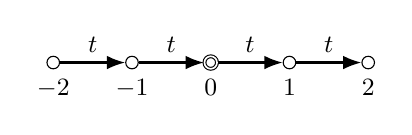
\begin{tikzpicture}[scale=1]
\node[vtx,label=below:$-2$] (m2) at (-2,0) {};
\node[vtx,label=below:$-1$] (m1) at (-1,0) {};
\node[basevtx,label=below:$0$] (z0) at (0,0) {};
\node[vtx,label=below:$1$] (p1) at (1,0) {};
\node[vtx,label=below:$2$] (p2) at (2,0) {};
\draw[edge] (m2) -- node[above]{$t$} (m1);
\draw[edge] (m1) -- node[above]{$t$} (z0);
\draw[edge] (z0) -- node[above]{$t$} (p1);
\draw[edge] (p1) -- node[above]{$t$} (p2);
\end{tikzpicture}
\caption{A finite window in $\Cay(\mathbb Z,\{t\})$. Reverse edges carry label $t^{-1}$.}
\end{figure}

\subsection*{Example 2: $\mathbb Z^2=\langle a,b\mid [a,b]\rangle$ (a grid)}
\paragraph{Forward construction (Algorithm A).}
\begin{enumerate}[leftmargin=2.2em]
\item Choose normal form: elements are pairs $(i,j)\in\mathbb Z^2$.
\item Vertices: one vertex for each $(i,j)$.
\item For each $(i,j)$, add the edge $(i,j)\xrightarrow{a}(i+1,j)$.
\item For each $(i,j)$, add the edge $(i,j)\xrightarrow{b}(i,j+1)$.
\item Reverse edges are labeled $a^{-1}$ and $b^{-1}$.
\end{enumerate}

\paragraph{Inverse reconstruction (Algorithm B).}
Assume you are given the labeled grid and basepoint $e=(0,0)$.
\begin{enumerate}[leftmargin=2.2em]
\item Compute $\End(ab)$: from $(0,0)$ go right via $a$ to $(1,0)$, then up via $b$ to $(1,1)$.
So $\End(ab)=(1,1)$.
\item Compute $\End(ba)$: from $(0,0)$ go up via $b$ to $(0,1)$, then right via $a$ to $(1,1)$.
So $\End(ba)=(1,1)$.
\item Therefore $\End(ab)=\End(ba)$, so $\End(aba^{-1}b^{-1})=e$.
Thus the commutator word labels a loop at $e$, hence $[a,b]\in N$.
\item The set of all square-boundary loops generate all loops in the grid, so $N=\langle\!\langle [a,b]\rangle\!\rangle$ and
$G\cong \langle a,b\mid [a,b]\rangle\cong\mathbb Z^2$.
\end{enumerate}

\begin{figure}[h]
\centering
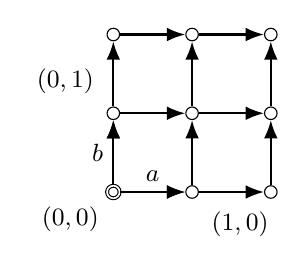
\begin{tikzpicture}[scale=1]
% vertices
\foreach \i in {0,1,2} {
  \foreach \j in {0,1,2} {
    \node[vtx] (v\i\j) at (\i,\j) {};
  }
}
\node[basevtx,label=below left:{$(0,0)$}] at (v00) {};
\node[label=below right:{$(1,0)$}] at (v10) {};
\node[label=above left:{$(0,1)$}] at (v01) {};
% edges
\foreach \i in {0,1} {
  \foreach \j in {0,1,2} {
    \draw[edge] (v\i\j) -- (v\the\numexpr\i+1\relax\j);
  }
}
\foreach \i in {0,1,2} {
  \foreach \j in {0,1} {
    \draw[edge] (v\i\j) -- (v\i\the\numexpr\j+1\relax);
  }
}
% labels on representative edges
\draw[edge] (v00) -- node[above]{$a$} (v10);
\draw[edge] (v00) -- node[left]{$b$} (v01);
\end{tikzpicture}
\caption{A finite patch of $\Cay(\mathbb Z^2,\{a,b\})$ (all horizontal edges labeled $a$, all vertical edges labeled $b$).}
\end{figure}

\subsection*{Example 3: $F_2=\langle a,b\rangle$ (a tree)}
\paragraph{Forward construction (Algorithm A).}
\begin{enumerate}[leftmargin=2.2em]
\item Choose normal form: each element of $F(a,b)$ is a reduced word in $\{a^{\pm1},b^{\pm1}\}$.
\item Vertices: all reduced words $w$.
\item For each vertex $w$ and generator $x\in\{a^{\pm1},b^{\pm1}\}$:
compute $\mathrm{red}(wx)$ and add the edge $w\xrightarrow{x}\mathrm{red}(wx)$.
\item This produces a $4$-regular tree because reduced words have unique reduced prefixes and no cycles occur.
\end{enumerate}

\paragraph{Inverse reconstruction (Algorithm B).}
\begin{enumerate}[leftmargin=2.2em]
\item In a tree, any reduced closed path would create a cycle, impossible. Hence the only reduced loop is trivial.
\item Therefore $N=\{1\}$ and $G\cong F(a,b)$ is free.
\end{enumerate}

\begin{figure}[h]
\centering
\begin{tikzpicture}[scale=1, every node/.style={font=\scriptsize}]
\node[basevtx,label=below:$1$] (e) at (0,0) {};
\node[vtx,label=below:$a$] (a) at (2,0) {};
\node[vtx,label=below:$a^{-1}$] (ai) at (-2,0) {};
\node[vtx,label=left:$b$] (b) at (0,2) {};
\node[vtx,label=left:$b^{-1}$] (bi) at (0,-2) {};
\draw[edge] (e) -- node[above]{$a$} (a);
\draw[edge] (e) -- node[above]{$a^{-1}$} (ai);
\draw[edge] (e) -- node[left]{$b$} (b);
\draw[edge] (e) -- node[left]{$b^{-1}$} (bi);
% extend one branch
\node[vtx,label=below:$a^2$] (a2) at (4,0) {};
\node[vtx,label=above right:$ab$] (ab) at (3,1.5) {};
\draw[edge] (a) -- node[above]{$a$} (a2);
\draw[edge] (a) -- node[right]{$b$} (ab);
\end{tikzpicture}
\caption{A small ball in $\Cay(F_2,\{a,b\})$. Extending produces an infinite $4$-regular tree.}
\end{figure}

% ============================================================
\clearpage
\section{Subgroup graph (Stallings graph)}

\subsection*{Definition}
Let $F(X)$ be a free group on $X$ and $H\le F(X)$ a finitely generated subgroup.
A \emph{Stallings graph} for $H$ is a finite connected based folded $X$-labeled graph $(\Gamma_H,*)$
such that reduced loops at $*$ label exactly the elements of $H$\cite{stallings1983,kapovichmyasnikov2002}:
\[
H=\{\lab(p)\in F(X)\mid p\text{ is a reduced loop at }*\text{ in }\Gamma_H\}.
\]

\subsection*{Existence/uniqueness (precise statement)}
\begin{theorem}[Stallings graph: existence, algorithmic construction, and uniqueness]\label{thm:stallings}
Fix a basis $X$ of the free group $F(X)$ and let $H\le F(X)$ be finitely generated.
\begin{enumerate}[leftmargin=2.2em]
\item (\textbf{Existence}) There exists a finite connected based folded $X$-labeled graph $(\Gamma_H,*)$
such that the reduced loop language at $*$ equals $H$.

\item (\textbf{Cover interpretation}) Let $R_X$ be the rose with $|X|$ loops labeled by $X$.
Then $H$ corresponds to a based covering $p:\widetilde R\to R_X$ and $\Gamma_H$ is the \emph{finite core} of $\widetilde R$
(obtained by deleting all hanging trees not containing the basepoint).

\item (\textbf{Algorithmic construction}) Given any finite generating set $H=\langle w_1,\dots,w_m\rangle$,
the \emph{folding + pruning} algorithm (Algorithm~A below) terminates and outputs a graph isomorphic to $(\Gamma_H,*)$.

\item (\textbf{Uniqueness}) The isomorphism class of $(\Gamma_H,*)$ depends only on $H$ (and the fixed basis $X$),
not on the chosen generating set and not on the order in which folds are performed.

\item (\textbf{Consequences that are read off from $\Gamma_H$})
\begin{itemize}[leftmargin=2em]
\item Membership: $w\in H$ iff the reduced word $w$ labels a loop at $*$ in $\Gamma_H$.
\item Rank: $\mathrm{rank}(H)=|E(\Gamma_H)|-|V(\Gamma_H)|+1$.
\item Finite index: $H$ has finite index in $F(X)$ iff $\Gamma_H\to R_X$ is a covering (equivalently: each vertex has exactly one outgoing edge labeled $x$ for each $x\in X$).
If so, $[F(X):H]=|V(\Gamma_H)|$.
\end{itemize}
\end{enumerate}
\end{theorem}

\subsection*{Algorithm A (Forward): generators $\to$ Stallings graph (detailed)}\cite{stallings1983,kapovichmyasnikov2002,touikan2006}
\paragraph{Input.}
Freely reduced words $w_1,\dots,w_m\in (X^{\pm1})^*$ generating $H=\langle w_1,\dots,w_m\rangle\le F(X)$.

\paragraph{Output.}
The folded core graph $(\Gamma_H,*)$.

\paragraph{Data structure convention.}
We view $\Gamma$ as:
\begin{itemize}[leftmargin=2em]
\item a set of vertices $V$ with a distinguished basepoint $*$,
\item for each vertex $v$ and label $a\in X^{\pm1}$, a (partial) map \texttt{out}[v,a] giving the unique outgoing $a$-edge if it exists,
\item and each edge stores its initial and terminal vertices and its label.
\end{itemize}

\paragraph{Steps.}
\begin{enumerate}[leftmargin=2.2em]
\item \textbf{Free-reduce the inputs.}
Replace each $w_i$ by its freely reduced form. (This does not change the subgroup they generate.)

\item \textbf{Build the bouquet-of-words graph $\Gamma_0$.}
\begin{enumerate}[leftmargin=2em]
\item Initialize $\Gamma$ with one vertex $*$.
\item For each word $w_i=a_1a_2\cdots a_k$ with $a_j\in X^{\pm1}$:
create a path of $k$ directed edges labeled $a_1,\dots,a_k$ starting at $*$ and ending at $*$.
Concretely, create new intermediate vertices $v_1,\dots,v_{k-1}$, and edges
\[
* \xrightarrow{a_1} v_1 \xrightarrow{a_2}\cdots\xrightarrow{a_k} *.
\]
\end{enumerate}

\item \textbf{Fold until deterministic.}
Maintain a queue of \emph{fold candidates}:
pairs of distinct edges $(e_1,e_2)$ with the same initial vertex and the same label.
While the queue is nonempty:
\begin{enumerate}[leftmargin=2em]
\item Pop a candidate $(e_1,e_2)$ with $\iota(e_1)=\iota(e_2)=v$ and $\lab(e_1)=\lab(e_2)=a$.
\item \textbf{Perform the fold:} identify $e_1$ and $e_2$ into one edge, and identify their terminal vertices $\tau(e_1)$ and $\tau(e_2)$.
This is a quotient operation on the graph.
\item \textbf{Update adjacency:} whenever vertices are identified, merge their outgoing edge tables.
If merging creates new duplicates (same label leaving the merged vertex), add them to the queue.
\item Continue until no duplicate-labeled outgoing edges remain anywhere.
\end{enumerate}
The resulting labeled graph is folded/deterministic; call it $\Gamma_{\mathrm{fold}}$.

\item \textbf{Prune to the core.}
Compute degrees in the underlying undirected graph.
While there exists a vertex $v\neq *$ of degree $1$:
\begin{enumerate}[leftmargin=2em]
\item remove $v$ and its unique incident edge,
\item update degrees of its neighbor,
\item repeat until no such vertex remains.
\end{enumerate}
The remaining graph is the \emph{core} $\Gamma_H$.
\end{enumerate}

\paragraph{Correctness summary (what the algorithm guarantees).}
\begin{itemize}[leftmargin=2em]
\item Every $w_i$ labels a loop at $*$ in $\Gamma_H$ (by construction).
\item Folding does not change the subgroup recognized by loops at $*$ (it identifies indistinguishable states).
\item Pruning removes only hanging trees that do not contribute to based loops, so the loop language is unchanged.
\end{itemize}

\paragraph{Boundary cases and implementation notes.}
\begin{itemize}[leftmargin=2em]
\item \textbf{Already folded input.} If $\Gamma_0$ is already folded (no vertex has two outgoing edges with the same label), then the fold-candidate queue is empty and the folding loop does nothing. The algorithm proceeds directly to pruning.
\item \textbf{Trivial subgroup.} If $m=0$ (no generators) or all $w_i$ freely reduce to the empty word, then $\Gamma_0$ is a single vertex $*$ with no edges. Folding and pruning do nothing and the output Stallings graph is the single base vertex; it recognizes exactly $H=\{1\}$.
\item \textbf{Whole group.} If the input generators contain $X$ itself (e.g.\ $H=\langle X\rangle=F(X)$), then the output core is the rose $R_X$ (one vertex with one loop for each $x\in X$).
\item \textbf{Keep the basepoint.} During pruning, never delete the basepoint $*$ even if it temporarily has degree $1$; otherwise you would destroy the based-loop language.
\end{itemize}

\paragraph{Complexity (one standard bound; not necessarily optimal).}\cite{stallings1983,touikan2006,tarjan1975}
Let $L=\sum_{i=1}^m |w_i|$ after free reduction.
\begin{itemize}[leftmargin=2em]
\item \textbf{Building $\Gamma_0$.} Time $O(L)$ and space $O(L)$ vertices/edges.
\item \textbf{Folding (naive).} If you implement folding by repeatedly scanning for conflicts, a safe bound is $O(L^2)$ time in the worst case.
\item \textbf{Folding (typical efficient implementation).} Using union-find for vertex identifications and hash tables for \texttt{out}[v,a], one can achieve near-linear time, e.g.\ $O(L\alpha(L))$ or $O(L\log L)$, and $O(L)$ space.
\item \textbf{Pruning to the core.} Time $O(|V|+|E|)=O(L)$ with a queue of degree-$1$ vertices; space $O(L)$.
\end{itemize}


\subsection*{Algorithm B (Inverse): Stallings graph $\to$ subgroup data (detailed)}\cite{stallings1983,kapovichmyasnikov2002,touikan2006}
\paragraph{Input.}
A finite based folded labeled graph $(\Gamma,*)$.

\paragraph{Outputs.}
\begin{itemize}[leftmargin=2em]
\item The subgroup $H\le F(X)$ recognized by loops at $*$.
\item An explicit free basis of $H$ (Schreier basis relative to a chosen tree).
\item Membership/coset-state computation for words.
\end{itemize}

\paragraph{Steps.}
\begin{enumerate}[leftmargin=2.2em]
\item \textbf{Recover $H$ as a loop language.}
Define:
\[
H(\Gamma)=\{\lab(p)\in F(X)\mid p\text{ is a reduced loop at }*\}.
\]
This is a subgroup because concatenation of loops corresponds to multiplication in $F(X)$.

\item \textbf{Membership test (deterministic traversal).}
Given a reduced word $w=a_1\cdots a_k$:
\begin{enumerate}[leftmargin=2em]
\item set current vertex $v\leftarrow *$,
\item for $j=1,\dots,k$: if there is an outgoing edge from $v$ labeled $a_j$, traverse it and update $v$; otherwise stop and declare $w\notin H$,
\item after reading all letters, declare $w\in H$ iff $v=*$.
\end{enumerate}

\item \textbf{Compute a free basis via a spanning tree.}
\begin{enumerate}[leftmargin=2em]
\item Choose a maximal spanning tree $T$ of the underlying undirected graph of $\Gamma$.
(For algorithmic purposes, choose the BFS tree from $*$.)
\item For each vertex $v$, let $\sigma(v)$ be the label of the unique reduced path in $T$ from $*$ to $v$.
\item For each oriented edge $e$ not in $T$ (choose one orientation per undirected edge), output the word
\[
g_e=\sigma(\iota(e))\,\lab(e)\,\sigma(\tau(e))^{-1}.
\]
\item Then $\{g_e: e\notin T\}$ is a free basis of $H(\Gamma)$.
\end{enumerate}

\item \textbf{Compute rank and (if finite index) the index.}
\begin{enumerate}[leftmargin=2em]
\item Rank: $|E|-|V|+1$.
\item Check covering condition: for each vertex $v$ and each $x\in X$, verify exactly one outgoing $x$-edge.
If true, index is $|V|$.
\end{enumerate}
\end{enumerate}



\paragraph{Boundary cases and choices.}
\begin{itemize}[leftmargin=2em]
\item \textbf{Trivial subgroup.} If $\Gamma$ has one vertex and no edges, then $H=\{1\}$ and the Schreier basis is empty (rank $0$).
\item \textbf{Non-folded input.} If $\Gamma$ is not folded, then reading a word from $*$ may have multiple paths; membership is not decidable by deterministic traversal. In practice you fold first (Algorithm~A) or determinize the graph.
\item \textbf{Choice of spanning tree.} Different choices of spanning tree $T$ produce different Schreier bases; these bases are all free bases of the same subgroup and are related by Nielsen transformations. (The subgroup itself is independent of $T$.)
\end{itemize}

\paragraph{Complexity (rough).}\cite{stallings1983,schreier1927,cormen2009}
Let $\Gamma$ be finite with $|V|$ vertices and $|E|$ directed edges (or count undirected edges and multiply by $2$).
\begin{itemize}[leftmargin=2em]
\item \textbf{Spanning tree.} Build a spanning tree by DFS/BFS in $O(|V|+|E|)$ time and $O(|V|)$ space.
\item \textbf{Compute $\sigma(v)$.} If you store parent pointers in the tree, computing all $\sigma(v)$ as \emph{paths} costs $O(|V|)$.
If you materialize $\sigma(v)$ as explicit words, the total output size can be $O(|V|^2)$ in the worst case, because some tree paths may have length $\Theta(|V|)$.
\item \textbf{Schreier basis.} There are $|E|-|V|+1$ non-tree edges, so basis size is $|E|-|V|+1$.
Computing each $g_e$ costs time proportional to the length of the corresponding tree paths (or $O(1)$ if you keep them as paths).
\item \textbf{Membership.} Given a reduced word $w$ of length $n$, deterministic traversal takes $O(n)$ time and $O(1)$ extra space.
\end{itemize}
\subsection*{Worked example 1: $H=\langle a^2,b\rangle\le F(a,b)$ (no folds occur)}
\paragraph{Forward construction (Algorithm A).}
\begin{enumerate}[leftmargin=2.2em]
\item Inputs: $w_1=a^2=aa$, $w_2=b$ (already freely reduced).
\item Build $\Gamma_0$:
\begin{enumerate}[leftmargin=2em]
\item Start with basepoint vertex $*$.
\item For $aa$: create one new vertex $v$ and edges $*\xrightarrow{a}v$ and $v\xrightarrow{a}*$.
\item For $b$: add a loop edge $*\xrightarrow{b}*$.
\end{enumerate}
\item Folding stage: check outgoing edges.
At $*$ there is one $a$-edge and one $b$-edge; at $v$ there is one $a$-edge. No duplicate labels, so no folds.
\item Pruning stage: degrees are $\deg(v)=2$ and $\deg(*)\ge 2$, hence no removable leaves. So $\Gamma_H=\Gamma_0$.
\end{enumerate}

\paragraph{Inverse reconstruction (Algorithm B).}
\begin{enumerate}[leftmargin=2.2em]
\item Membership facts read off from traversal:
\begin{itemize}[leftmargin=2em]
\item $b$ labels a loop at $*$, so $b\in H$.
\item $aa$ labels the loop $*\xrightarrow{a}v\xrightarrow{a}*$, so $a^2\in H$.
\item $a$ ends at $v\neq *$, so $a\notin H$.
\end{itemize}
\item Basis via a spanning tree:
\begin{enumerate}[leftmargin=2em]
\item Choose $T$ containing the undirected edge between $*$ and $v$.
Then $\sigma(*)=\varepsilon$ and $\sigma(v)=a$.
\item The non-tree edges are:
the $b$-loop at $*$ and the edge $v\xrightarrow{a}*$.
\item Compute Schreier generators:
$g_{b\text{-loop}}=b$ and $g_{v\to *}=a\cdot a=a^2$.
\end{enumerate}
\end{enumerate}

\begin{figure}[h]
\centering
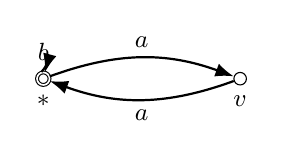
\begin{tikzpicture}[scale=1]
\node[basevtx,label=below:$*$] (s) at (0,0) {};
\node[vtx,label=below:$v$] (v) at (2.5,0) {};
% a-edges (two directed edges between s and v)
\draw[edge,bend left=20] (s) to node[above]{$a$} (v);
\draw[edge,bend left=20] (v) to node[below]{$a$} (s);
% b-loop at s
\draw[edge,loop above] (s) to node[above]{$b$} (s);
\end{tikzpicture}
\caption{Stallings graph for $H=\langle a^2,b\rangle\le F(a,b)$.}
\end{figure}

\subsection*{Worked example 2 (with an actual fold): $H=\langle a,ab\rangle\le F(a,b)$}
This example is useful because the fold step is \emph{nontrivial} and illustrates the algorithm mechanically.

\paragraph{Forward construction (Algorithm A).}
\begin{enumerate}[leftmargin=2.2em]
\item Inputs: $w_1=a$, $w_2=ab$ (already reduced).
\item Build $\Gamma_0$:
\begin{enumerate}[leftmargin=2em]
\item For $a$: add a loop edge $*\xrightarrow{a}*$.
\item For $ab$: create a new vertex $v$ and edges $*\xrightarrow{a}v$ and $v\xrightarrow{b}*$.
\end{enumerate}
\item Folding stage:
\begin{enumerate}[leftmargin=2em]
\item At the basepoint $*$ there are \emph{two} outgoing $a$-edges:
one is the $a$-loop with terminal $*$, the other is the first edge of the $ab$ path with terminal $v$.
\item Fold these two $a$-edges together. This identifies their terminal vertices, so $v$ is identified with $*$.
\item After this identification, the edge $v\xrightarrow{b}*$ becomes a $b$-loop at $*$.
\item Now at $*$ there is exactly one outgoing $a$-edge and one outgoing $b$-edge, so the graph is folded.
\end{enumerate}
\item Pruning stage: there are no degree-$1$ vertices. Output $\Gamma_H$ which is the rose with two loops labeled $a$ and $b$.
\end{enumerate}

\paragraph{Inverse reconstruction (Algorithm B).}
\begin{enumerate}[leftmargin=2.2em]
\item In the output graph, both $a$ and $b$ are loops at the basepoint, hence $a,b\in H$.
\item Therefore $H$ contains a free basis $\{a,b\}$ and so $H=F(a,b)$.
(Indeed, algebraically $b=a^{-1}(ab)\in \langle a,ab\rangle$.)
\end{enumerate}

\begin{figure}[h]
\centering
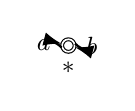
\begin{tikzpicture}[scale=1]
\node[basevtx,label=below:$*$] (s) at (0,0) {};
% loops a and b
\draw[edge,loop left] (s) to node[left]{$a$} (s);
\draw[edge,loop right] (s) to node[right]{$b$} (s);
\end{tikzpicture}
\caption{After folding, the Stallings graph for $\langle a,ab\rangle$ is the rose with two loops: this subgroup is all of $F(a,b)$.}
\end{figure}
\clearpage
% ============================================================
\section{Enriched subgroup graph (Stallings + marking)}

\subsection*{Definition}
An \emph{enriched subgroup graph} is a triple $(\Gamma_H,*,T)$ where:
\begin{itemize}[leftmargin=2em]
\item $(\Gamma_H,*)$ is the Stallings graph of $H\le F(X)$,
\item $T$ is a chosen maximal spanning tree of $\Gamma_H$ (undirected sense).
\end{itemize}
The enrichment provides \emph{explicit} Schreier generators, a preferred set of tree-words $\sigma(v)$, and a deterministic procedure to decompose elements of $H$ in a chosen free basis.\cite{schreier1927,stallings1983}

\subsection*{Existence/uniqueness (precise statement)}
\begin{proposition}[Enrichment exists; what is unique and what is not]\label{prop:enriched}
Let $H\le F(X)$ be finitely generated.
\begin{enumerate}[leftmargin=2.2em]
\item (\textbf{Existence}) The Stallings graph $(\Gamma_H,*)$ exists and is unique up to based label-preserving isomorphism (Theorem~\ref{thm:stallings}).
Every finite connected graph admits a maximal spanning tree, hence an enrichment $(\Gamma_H,*,T)$ always exists.

\item (\textbf{Non-uniqueness}) The tree $T$ is not canonical in general.
Different choices of $T$ typically yield different Schreier bases, though all such bases are Nielsen-equivalent.

\item (\textbf{Uniqueness relative to a chosen tree}) If $(\Gamma_H,*,T)$ and $(\Gamma_H,*,T')$ are two enrichments,
then they are isomorphic as enriched objects iff there exists a based label-preserving automorphism $\Phi$ of $\Gamma_H$ such that $\Phi(T)=T'$.
\end{enumerate}
\end{proposition}

\subsection*{Algorithm A (Forward): build and enrich (detailed)}\cite{schreier1927,stallings1983,serre1980trees}
\paragraph{Input.} Generators $w_1,\dots,w_m$ of $H\le F(X)$.
\paragraph{Output.} Enriched object $(\Gamma_H,*,T)$ plus the associated Schreier basis and tree-word table.

\paragraph{Steps.}
\begin{enumerate}[leftmargin=2.2em]
\item Build $(\Gamma_H,*)$ using the Stallings folding+pruning algorithm (Algorithm~A in the previous section).
\item Choose a maximal spanning tree $T$ of $\Gamma_H$ (for determinism, choose a BFS tree from $*$).
\item Compute the tree words:
for each vertex $v$, compute $\sigma(v)$ as the label of the unique path in $T$ from $*$ to $v$.
(Algorithmically: store parent pointers and edge labels in the BFS tree.)
\item For each oriented edge $e\notin T$, compute the Schreier generator
\[
g_e=\sigma(\iota(e))\,\lab(e)\,\sigma(\tau(e))^{-1}.
\]
\item Output the set $\mathcal B_T=\{g_e:e\notin T\}$ as a free basis of $H$.
\end{enumerate}


\paragraph{What changes if you choose a different spanning tree $T$? (non-uniqueness in a precise sense)}
The \emph{underlying} Stallings graph $(\Gamma_H,*)$ is canonical up to based label-preserving isomorphism.
However, the additional data of a spanning tree is a \emph{choice}:
\begin{itemize}[leftmargin=2em]
\item The tree determines the table of \emph{tree-words} $\sigma(v)$ (words in $X^{\pm1}$ reaching each vertex).
\item The Schreier generators are built from these $\sigma(v)$ via $g_e=\sigma(\iota(e))\lab(e)\sigma(\tau(e))^{-1}$.
So changing $T$ changes $\sigma(\cdot)$ and therefore changes the \emph{explicit} basis $\mathcal B_T$.
\item Different $\mathcal B_T$ are bases of the same free group $H$, and any two such bases are related by Nielsen moves
(so they generate the same subgroup but give different coordinate systems).
\item Likewise, Algorithm~B produces different \emph{factorizations} of the same $w\in H$ depending on $T$.
\end{itemize}

\paragraph{Boundary cases.}
\begin{itemize}[leftmargin=2em]
\item If $\Gamma_H$ has a single vertex and no edges (so $H=\{1\}$), then $T$ is trivial and $\mathcal B_T=\varnothing$.
\item If $\Gamma_H$ is a tree (so $|E|=|V|-1$), then $\mathcal B_T=\varnothing$ and necessarily $H=\{1\}$ for a core subgroup graph.
\end{itemize}

\paragraph{Complexity (rough).}\cite{schreier1927,hatcher2002,cormen2009}
Let $\Gamma_H$ have $|V|$ vertices and $|E|$ directed edges.
\begin{itemize}[leftmargin=2em]
\item Choosing a BFS spanning tree and storing parent pointers costs $O(|V|+|E|)$ time and $O(|V|)$ space.
\item Computing all $\sigma(v)$ as parent-pointer paths costs $O(|V|)$ (but writing them out as explicit words can cost $O(|V|^2)$ total output length in the worst case).
\item Computing all Schreier generators $g_e$ costs $O(|E|)$ operations \emph{plus} the cost of materializing the tree-words used in the formula.
\end{itemize}

\subsection*{Algorithm B (Inverse): membership \emph{and} explicit decomposition (detailed)}\cite{schreier1927,stallings1983,serre1980trees}
\paragraph{Input.} An enriched graph $(\Gamma,*,T)$ and a word $w\in (X^{\pm1})^*$.
\paragraph{Output.}
Either a certificate that $w\notin H$, or a decomposition of $w$ as a word in the Schreier basis $\mathcal B_T$.

\paragraph{Steps.}
\begin{enumerate}[leftmargin=2.2em]
\item Freely reduce $w$.
\item Deterministic traversal:
\begin{enumerate}[leftmargin=2em]
\item set $v_0\leftarrow *$,
\item for each letter $a_i$ of $w$, traverse the unique outgoing edge labeled $a_i$ if it exists; if it does not exist, stop and output ``$w\notin H$ (path undefined)''.
Let $v_i$ be the vertex after reading the first $i$ letters.
\end{enumerate}
\item If $v_{|w|}\neq *$, output ``$w\notin H$ (endpoint is $v_{|w|}$)''.
\item If $v_{|w|}=*$, then $w\in H$. To compute a decomposition:
\begin{enumerate}[leftmargin=2em]
\item Initialize an empty word $W$ in the alphabet $\mathcal B_T^{\pm1}$.
\item For each traversed edge $e_i:v_{i-1}\xrightarrow{a_i}v_i$:
\begin{itemize}[leftmargin=2em]
\item if the undirected edge underlying $e_i$ lies in the tree $T$, record nothing (tree edges belong to the transversal part);
\item if the undirected edge is \emph{not} in $T$, then:
\begin{enumerate}[leftmargin=2em]
\item determine the chosen orientation $e$ for that non-tree undirected edge (the one used to define $g_e$),
\item if $e_i=e$, append $g_e$ to $W$; if $e_i=\overline e$ append $g_e^{-1}$ to $W$.
\end{enumerate}
\end{itemize}
\item Output $W$. Then the element represented by $W$ in the free group on $\mathcal B_T$ equals the element represented by $w$ in $H$.
\end{enumerate}
\end{enumerate}



\paragraph{Boundary cases and output format.}
\begin{itemize}[leftmargin=2em]
\item \textbf{Empty word.} If $w=\varepsilon$, traversal stays at $*$ and the decomposition output is the empty product (the identity of $H$).
\item \textbf{Traversal fails early.} If at step $i$ there is no outgoing edge labeled $a_i$, then you can output the partial endpoint $v_{i-1}$ as a ``coset-state'' and the failing letter $a_i$ as an explicit certificate that $w\notin H$ in this deterministic automaton.
\item \textbf{Endpoint not basepoint.} If traversal succeeds but ends at $v\neq *$, then $w\notin H$ and $v$ records the state reached by $w$.
\end{itemize}

\paragraph{Complexity (rough).}\cite{schreier1927,hatcher2002,cormen2009}
Let $n=|w|$.
\begin{itemize}[leftmargin=2em]
\item Deterministic traversal costs $O(n)$ time (one outgoing-edge lookup per letter) and $O(1)$ auxiliary space.
\item If you store a boolean ``is-tree-edge'' for each undirected edge, then deciding whether to output $g_e^{\pm1}$ at each step is $O(1)$.
\item The produced factorization has length at most $n$ (you output at most one basis letter per traversed edge), so output size is $O(n)$.
\end{itemize}
\subsection*{Worked example: enrichment for $H=\langle a^2,b\rangle$}
We reuse the Stallings graph in Worked example~1 of the previous section.

\paragraph{Forward enrichment (Algorithm A).}
\begin{enumerate}[leftmargin=2.2em]
\item Choose the spanning tree $T$ containing the undirected $a$-edge between $*$ and $v$.
\item Compute tree words: $\sigma(*)=\varepsilon$ and $\sigma(v)=a$.
\item Non-tree edges:
\begin{itemize}[leftmargin=2em]
\item the $b$-loop at $*$ gives $g_b=b$,
\item the edge $v\xrightarrow{a}*$ gives $g_{a}=a\cdot a=a^2$.
\end{itemize}
So $\mathcal B_T=\{b,a^2\}$.
\end{enumerate}

\paragraph{Inverse use (Algorithm B): decide membership and decompose $w=b\,a^2\,b^{-1}$.}
\begin{enumerate}[leftmargin=2.2em]
\item $w$ is already freely reduced.
\item Traverse:
\[
*\xrightarrow{b}*\xrightarrow{a}v\xrightarrow{a}*\xrightarrow{b^{-1}}*.
\]
So endpoint is $*$ and $w\in H$.
\item Decompose using $T$:
\begin{itemize}[leftmargin=2em]
\item The first edge is the non-tree $b$-loop: record $b$.
\item The next edge $*\xrightarrow{a}v$ is a tree edge: record nothing.
\item The next edge $v\xrightarrow{a}*$ is non-tree: record $a^2$.
\item The last edge is the inverse of the $b$-loop: record $b^{-1}$.
\end{itemize}
Hence $w=b\,(a^2)\,b^{-1}$ in the Schreier basis.
\end{enumerate}

\begin{figure}[h]
\centering
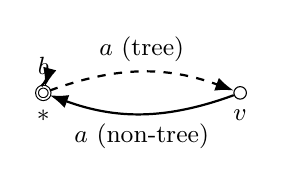
\begin{tikzpicture}[scale=1]
\node[basevtx,label=below:$*$] (s) at (0,0) {};
\node[vtx,label=below:$v$] (v) at (2.5,0) {};
% tree edge (dashed)
\draw[treedge,-Latex,bend left=20] (s) to node[above]{$a$ (tree)} (v);
% non-tree a edge
\draw[nonte,edge,bend left=20] (v) to node[below]{$a$ (non-tree)} (s);
% b-loop (non-tree)
\draw[nonte,edge,loop above] (s) to node[above]{$b$} (s);
\end{tikzpicture}
\caption{Enriched subgroup graph: dashed edge is the chosen spanning-tree edge. Non-tree edges give Schreier basis elements.}
\end{figure}

% ============================================================
\clearpage
\section{Schreier coset graph}

\subsection*{Definition}
Let $G$ be generated by $S$ and let $H\le G$.
The \emph{Schreier coset graph} $\Sch(G,H,S)$ has:
\begin{itemize}[leftmargin=2em]
\item vertices: right cosets $Hg$,
\item edges: $Hg\xrightarrow{s}Hgs$ for each $s\in S$.
\end{itemize}
The base vertex is $H$.\cite{schreier1927,serre1980trees}

\subsection*{Existence/uniqueness (precise statement)}
\begin{theorem}[Schreier graphs: existence and uniqueness]\label{thm:schreier}
Fix $(G,H,S)$.
\begin{enumerate}[leftmargin=2.2em]
\item (\textbf{Existence}) $\Sch(G,H,S)$ exists. It is finite iff $[G:H]<\infty$.
\item (\textbf{Uniqueness}) The based labeled graph $\Sch(G,H,S)$ is uniquely determined up to based label-preserving isomorphism by the marked data $(G,H,S)$.
\item (\textbf{Free-group covering classification}) If $G=F(X)$, then $\Sch(F(X),H,X)$ is the 1-skeleton of the covering of the rose $R_X$ corresponding to $H$.
Thus the Schreier graph is unique up to based labeled isomorphism because connected based coverings of $R_X$ are classified by subgroups of $\pi_1(R_X)\cong F(X)$.
\end{enumerate}
\end{theorem}

\subsection*{Algorithm A (Forward): build Schreier graph (detailed)}\cite{schreier1927,toddcoxeter1936,serre1980trees,holt2005}
\paragraph{Input.} A group $G$, subgroup $H$, generating set $S$.

\paragraph{Output.}
A directed labeled graph with vertex set $H\backslash G$.

\paragraph{Steps (conceptual).}
\begin{enumerate}[leftmargin=2.2em]
\item Enumerate the set of cosets $\{Hg\}$.
(If $[G:H]$ is finite, a coset enumeration algorithm such as Todd--Coxeter can produce the coset table.)
\item Create one vertex for each coset.
\item For each coset vertex $Hg$ and each $s\in S$, compute the product coset $Hgs$ and add the directed edge $Hg\xrightarrow{s}Hgs$.
\end{enumerate}


\paragraph{Boundary cases.}
\begin{itemize}[leftmargin=2em]
\item \textbf{$H=G$.} There is exactly one coset, so $\Sch(G,G,S)$ is a single vertex with a loop for each $s\in S$.
\item \textbf{$H=\{1\}$.} Cosets are singletons, so $\Sch(G,\{1\},S)$ is exactly the Cayley graph $\Cay(G,S)$.
\item \textbf{Non-generating $S$.} If $S$ does not generate $G$, the Schreier graph decomposes into multiple connected components corresponding to cosets of $\langle S\rangle$; we usually assume $S$ generates.
\end{itemize}

\paragraph{Uniqueness vs.\ ``choice of representatives'' (what can change and what cannot).}
The \emph{definition} uses vertices equal to the cosets $Hg$, so the Schreier graph is canonical up to based label-preserving isomorphism (Theorem~\ref{thm:schreier}).
However, in computations and drawings one often labels a vertex by a \emph{chosen representative word} $\widehat g$ for the coset $Hg$.
If you change representatives (e.g.\ replace $\widehat g$ by $h\widehat g$ with $h\in H$), then:
\begin{itemize}[leftmargin=2em]
\item the \textbf{vertex names} change,
\item the abstract labeled graph \textbf{does not change} (you only applied a relabeling of vertices),
\item any two such ``representative-labeled'' drawings are related by a label-preserving graph isomorphism that sends one chosen transversal to the other.
\end{itemize}

\paragraph{Complexity (rough).}\cite{schreier1927,toddcoxeter1936,holt2005}
Let $m=[G:H]$ if finite.
\begin{itemize}[leftmargin=2em]
\item If a coset table is available (i.e.\ you can compute $Hg\cdot s$ for each coset and each $s\in S$), then constructing the Schreier graph takes $O(m|S|)$ time and stores $O(m|S|)$ directed edges.
\item Producing the coset table itself (Todd--Coxeter) can be expensive in the worst case; we do not claim an optimal bound here.
\end{itemize}

\subsection*{Algorithm B (Inverse): membership and Schreier generators (detailed)}\cite{schreier1927,toddcoxeter1936,serre1980trees,holt2005}
\paragraph{Input.} A Schreier graph $\Sch(G,H,S)$ with base vertex $H$.
\paragraph{Output.} Membership test, coset reached by a word, and (optionally) Schreier generators for $H$.

\paragraph{Steps.}
\begin{enumerate}[leftmargin=2.2em]
\item \textbf{Membership and coset output.}
Given a word $w=s_1\cdots s_k$ in $S^{\pm1}$:
\begin{enumerate}[leftmargin=2em]
\item start at vertex $v_0=H$,
\item follow the unique edge labeled $s_i$ at each step (Schreier graphs are complete in the labels),
\item end at vertex $v_k=Hw$.
\end{enumerate}
Then $w\in H$ iff $v_k=H$.

\item \textbf{Schreier generators from a spanning tree.}
\begin{enumerate}[leftmargin=2em]
\item Choose a spanning tree $T$ of the (undirected) Schreier graph.
\item For each vertex $v$, define $\sigma(v)$ as the label of the unique tree path in $T$ from $H$ to $v$.
\item For each directed edge $e:v\xrightarrow{s}w$ not in $T$, output
\[
g_e=\sigma(v)\,s\,\sigma(w)^{-1}\in H.
\]
These elements generate $H$ (and in free-group settings yield a free basis).
\end{enumerate}
\end{enumerate}



\paragraph{Boundary cases and choices.}
\begin{itemize}[leftmargin=2em]
\item \textbf{Membership is always well-defined.} Schreier graphs are complete in the labels: from each coset $Hg$ and generator $s\in S$ there is an edge labeled $s$.
So reading a word is always possible and ends at a well-defined coset.
\item \textbf{Choice of spanning tree.} The Schreier generator formula depends on the choice of spanning tree $T$ (equivalently, on the choice of a coset transversal $\{\sigma(v)\}$).
Changing $T$ changes the specific generating set produced, but not the subgroup $H$.
\end{itemize}

\paragraph{Complexity (rough).}\cite{schreier1927,serre1980trees,cormen2009}
\begin{itemize}[leftmargin=2em]
\item \textbf{Membership / coset reached.} For a word $w$ of length $n$, traversal takes $O(n)$ time and $O(1)$ extra space (besides the stored graph).
\item \textbf{Schreier generators (finite index $m$).} Choosing a spanning tree takes $O(m|S|)$ time on the Schreier graph, and generating the list of non-tree edges is $O(m|S|)$.
\end{itemize}
\subsection*{Worked example: $G=\mathbb Z=\langle t\rangle$, $H=2\mathbb Z$}
\paragraph{Forward construction (Algorithm A).}
\begin{enumerate}[leftmargin=2.2em]
\item The subgroup $H=2\mathbb Z$ has index $2$, so there are two right cosets.
\item Representatives: $H$ (even integers) and $Ht$ (odd integers).
\item Create vertices $v_0=H$ and $v_1=Ht$.
\item For generator $t$:
\[
H\xrightarrow{t}Ht,\qquad Ht\xrightarrow{t}Ht^2=H.
\]
\end{enumerate}

\paragraph{Inverse reconstruction (Algorithm B).}
\begin{enumerate}[leftmargin=2.2em]
\item Reading a word $t^k$ from base vertex $H$ toggles between the two cosets.
\item Therefore $t^k\in H$ iff $k$ is even, hence $H=\langle t^2\rangle$.
\item If we choose the spanning tree $T$ containing the edge $H\xrightarrow{t}Ht$, then $\sigma(H)=\varepsilon$, $\sigma(Ht)=t$,
and the non-tree edge $Ht\xrightarrow{t}H$ gives Schreier generator $t\cdot t=t^2$.
\end{enumerate}

\begin{figure}[h]
\centering
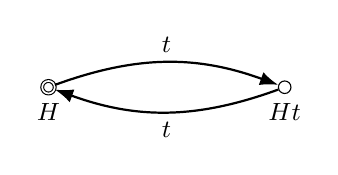
\begin{tikzpicture}[scale=1]
\node[basevtx,label=below:$H$] (H) at (0,0) {};
\node[vtx,label=below:$Ht$] (Ht) at (3,0) {};
\draw[edge,bend left=20] (H) to node[above]{$t$} (Ht);
\draw[edge,bend left=20] (Ht) to node[below]{$t$} (H);
\end{tikzpicture}
\caption{Schreier graph $\Sch(\mathbb Z,2\mathbb Z,\{t\})$. Reverse edges carry $t^{-1}$.}
\end{figure}

% ============================================================
\section{Disk diagram}

\subsection*{Definition}
A \emph{disk diagram} over a 2-complex $X$ is a finite 2-complex $D$ equipped with a combinatorial map $D\to X$
whose underlying topological space is a disk.
Its boundary $\partial D$ is a single combinatorial cycle; if edges are labeled, $\partial D$ has a boundary word.\cite{vanKampen1933,lyndonschupp1977}

\subsection*{Existence/uniqueness (precise statement)}
\begin{theorem}[Disk diagrams exist exactly for null-homotopic loops]\label{thm:disk-existence}
Let $X$ be a combinatorial 2-complex and let $\gamma$ be a combinatorial loop in $X$ (or a boundary word in a presentation setting).
\begin{enumerate}[leftmargin=2.2em]
\item (\textbf{Existence}) $\gamma$ is null-homotopic in $X$ if and only if there exists a disk diagram $D\to X$ with boundary mapping to $\gamma$.
\item (\textbf{Minimal area exists}) If at least one disk diagram exists, then there exists a disk diagram of minimal area,
where area means the number of 2-cells of $D$.
(This follows from the well-ordering of $\mathbb N$.)
\item (\textbf{Non-uniqueness}) Disk diagrams filling the same loop are generally not unique up to isomorphism, even among minimal-area fillings.
\end{enumerate}
\end{theorem}

\subsection*{Algorithm A (Forward): build a disk diagram (two detailed input types)}\cite{vanKampen1933,lyndonschupp1977}
\paragraph{Input type A1 (topological).} A null-homotopy $H:S^1\times[0,1]\to X$ of a loop $\gamma$.

\paragraph{Steps (A1).}
\begin{enumerate}[leftmargin=2.2em]
\item Identify the disk $D^2$ with $S^1\times[0,1]/(S^1\times\{1\}\text{ collapsed})$ so that $H$ induces a map $D^2\to X$.
\item Choose a triangulation (or polygonal cellulation) of $D^2$ that subdivides the boundary so the boundary map agrees with $\gamma$.
\item Apply cellular approximation to homotope the map to a combinatorial map sending vertices to vertices, edges to edge-paths, and faces to cellular 2-chains.
\item Record the resulting finite cell complex and map; this is the disk diagram.
\end{enumerate}

\paragraph{Input type A2 (presentation).}
A presentation $\mathcal P=\langle X\mid R\rangle$ and an explicit proof that a boundary word $w$ is trivial in $G(\mathcal P)$.

\paragraph{Steps (A2).}
\begin{enumerate}[leftmargin=2.2em]
\item Convert the proof into an equality in the free group:
\[
w=\prod_{i=1}^N u_i\, r_i^{\varepsilon_i}\,u_i^{-1}
\quad (r_i\in R,\;\varepsilon_i=\pm1).
\]
\item For each factor $r_i^{\varepsilon_i}$, create a polygonal 2-cell labeled by $r_i^{\varepsilon_i}$.
\item Attach a whisker path from a common boundary basepoint to the chosen start of the $i$th cell, labeled by $u_i$.
\item Glue boundary edges whenever adjacent letters cancel in the product; after gluing all cancellations, the remaining outer boundary reads $w$.
\item The result is a disk diagram; in the presentation case it is exactly a van Kampen diagram.
\end{enumerate}


\paragraph{Boundary cases.}
\begin{itemize}[leftmargin=2em]
\item \textbf{Trivial loop / empty word.} If $\gamma$ is homotopic to a constant loop (or $w$ freely reduces to the empty word), then the \emph{empty diagram} (no 2-cells, boundary length $0$) is a valid certificate.
\item \textbf{Already a single relator.} If $w$ is exactly a relator $r\in R^{\pm1}$, then a one-face polygon labeled by $r$ is a disk diagram.
\end{itemize}

\paragraph{Complexity (rough, for Input type A2).}\cite{vanKampen1933,lyndonschupp1977,tarjan1975}
Suppose you are given an explicit product-of-conjugates proof with total word length
\[
L_{\mathrm{proof}} := |w| + \sum_{i=1}^N \bigl(2|u_i|+|r_i|\bigr).
\]
\begin{itemize}[leftmargin=2em]
\item Creating the $N$ faces and whisker paths takes $O(L_{\mathrm{proof}})$ time and space.
\item Gluing cancellations can be done in $O(L_{\mathrm{proof}}\log L_{\mathrm{proof}})$ time using union-find / hashing on boundary arcs.
A very safe (non-optimized) bound for a naive implementation is $O(L_{\mathrm{proof}}^2)$ time.
\end{itemize}

\subsection*{Algorithm B (Inverse): disk diagram $\to$ explicit algebraic certificate (detailed)}\cite{vanKampen1933,lyndonschupp1977}
\paragraph{Input.} A disk diagram $D\to K(\mathcal P)$ with boundary word $w$.
\paragraph{Output.} A concrete expression $w=\prod u_f r_f^{\pm1}u_f^{-1}$ in the free group.

\paragraph{Steps.}
\begin{enumerate}[leftmargin=2.2em]
\item Choose a basepoint $*$ on the boundary $\partial D$.
\item Choose a spanning tree $T$ of the 1-skeleton $D^{(1)}$ that contains all boundary vertices (BFS tree works).
\item For each face $f$ of $D$:
\begin{enumerate}[leftmargin=2em]
\item choose a point $p_f$ on $\partial f$ (a vertex on its boundary),
\item let $u_f=\lab(\text{the unique path in }T\text{ from }*\text{ to }p_f)$,
\item read the cyclic word around $\partial f$ starting at $p_f$ in the direction consistent with the orientation; call it $r_f^{\varepsilon_f}$ (a relator or its inverse).
\end{enumerate}
\item Traverse the diagram in the plane to order the faces (any order works if you interpret multiplication in the free group carefully).
Then the boundary word satisfies
\[
w=\prod_{f\in \Faces(D)} u_f\, r_f^{\varepsilon_f}\,u_f^{-1}
\quad\text{in }F(X).
\]
\end{enumerate}



\paragraph{Boundary cases and correctness notes.}
\begin{itemize}[leftmargin=2em]
\item If $D$ has no faces, then $w$ must be freely trivial; the output product is empty.
\item The spanning tree choice affects the specific conjugators $u_f$, but not the fact that the product equals $w$ in $F(X)$.
\end{itemize}

\paragraph{Complexity (rough).}\cite{lyndonschupp1977,cormen2009}
Let $D$ have $|V|$ vertices, $|E|$ edges, $|F|$ faces, and total perimeter $P=\sum_f|\partial f|$.
\begin{itemize}[leftmargin=2em]
\item Building a spanning tree costs $O(|V|+|E|)$ time and $O(|V|)$ space.
\item Reading all face boundary words costs $O(P)$ time.
\item Therefore extracting a certificate costs $O(|V|+|E|+P)$ time.
\end{itemize}
\subsection*{Worked example: the commutator disk for $\langle a,b\mid aba^{-1}b^{-1}\rangle$}
\paragraph{Forward construction (Algorithm A2).}
\begin{enumerate}[leftmargin=2.2em]
\item Presentation: $\mathcal P=\langle a,b\mid r\rangle$ with $r=aba^{-1}b^{-1}$.
\item Boundary word: $w=r$.
\item Choose $N=1$, $u_1=\varepsilon$, $r_1=r$, $\varepsilon_1=+1$.
\item Create one square face whose boundary edges are labeled $a,b,a^{-1},b^{-1}$.
\item The outer boundary reads $w$, so this is a disk diagram for $w$.
\end{enumerate}

\paragraph{Inverse reconstruction (Algorithm B).}
\begin{enumerate}[leftmargin=2.2em]
\item Choose basepoint $*$ on the boundary (a corner of the square).
\item Choose spanning tree $T$ to be three edges of the square.
\item The diagram has one face $f$ with label $r$ and $u_f=\varepsilon$ (choose $p_f=*$).
\item Hence $w=u_f r u_f^{-1}=r$, so $w=1$ in $G(\mathcal P)$.
\end{enumerate}

\begin{figure}[h]
\centering
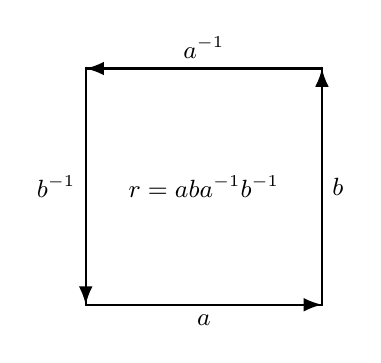
\begin{tikzpicture}[scale=1]
\coordinate (A) at (0,0);
\coordinate (B) at (3,0);
\coordinate (C) at (3,3);
\coordinate (D) at (0,3);
\draw[face] (A)--(B)--(C)--(D)--cycle;
\draw[edge] (A) -- node[below]{$a$} (B);
\draw[edge] (B) -- node[right]{$b$} (C);
\draw[edge] (C) -- node[above]{$a^{-1}$} (D);
\draw[edge] (D) -- node[left]{$b^{-1}$} (A);
\node at (1.5,1.5) {$r=aba^{-1}b^{-1}$};
\end{tikzpicture}
\caption{A disk diagram with one square face filling the commutator word.}
\end{figure}


\clearpage
% ============================================================
\section{Annular diagram}

\subsection*{Definition}
An \emph{annular diagram} over a 2-complex $X$ is a finite 2-complex $A\to X$ whose underlying space is an annulus.
It has two boundary components:
\[
\partial A=\partial_{\mathrm{out}}A\;\sqcup\;\partial_{\mathrm{in}}A,
\]
each a cycle carrying a cyclic boundary word.

\subsection*{Existence/uniqueness (precise statement)}
\begin{theorem}[Annular diagrams detect free homotopy and conjugacy]\label{thm:annulus}
\begin{enumerate}[leftmargin=2.2em]
\item (\textbf{Topological form}) Two loops $\gamma_0,\gamma_1:S^1\to X$ are freely homotopic in $X$
if and only if there exists an annular diagram $A\to X$ whose boundary components map to $\gamma_0$ and $\gamma_1$.
\item (\textbf{Group form}) For a presentation $\mathcal P=\langle X\mid R\rangle$ and cyclic words $u,v$ in $X^{\pm1}$,
$u$ and $v$ represent conjugate elements in $G(\mathcal P)$ if and only if there exists an annular van Kampen diagram over $\mathcal P$
with boundary labels $u$ and $v$ (up to cyclic rotation and orientation conventions).
\item (\textbf{Non-uniqueness}) Annular diagrams are generally not unique for fixed boundary data.
\end{enumerate}
\end{theorem}

\subsection*{Algorithm A (Forward): conjugacy $u=gvg^{-1}$ $\to$ annular diagram (detailed)}\cite{lyndonschupp1977}
\paragraph{Input.} A presentation $\mathcal P=\langle X\mid R\rangle$ and a conjugacy proof $u=gvg^{-1}$ in $G(\mathcal P)$.
\paragraph{Output.} An annular van Kampen diagram with boundary labels $u$ and $v$.

\paragraph{Steps.}
\begin{enumerate}[leftmargin=2.2em]
\item Form the word $W=gvg^{-1}u^{-1}$.
Then $W=1$ in $G(\mathcal P)$.
\item Construct a van Kampen disk diagram $D$ for $W$ (Algorithm A in the van Kampen section).
\item On $\partial D$, locate the subpath labeled $g$ and the subpath labeled $g^{-1}$.
(These appear as consecutive segments in the boundary word $gvg^{-1}u^{-1}$.)
\item Glue the $g$-subpath to the $g^{-1}$-subpath by identifying corresponding edges with opposite orientations.
\item After gluing, the boundary splits into two cycles labeled by $u$ and $v$ (as cyclic words).
The resulting complex is an annulus: an annular diagram.
\end{enumerate}

\paragraph{Boundary cases and conventions.}
\begin{itemize}[leftmargin=2em]
\item \textbf{Cyclic words.} The boundary labels of an annular diagram are \emph{cyclic} words: choosing a different basepoint on a boundary component cyclically rotates the boundary word. Reversing the orientation inverts the cyclic word.
\item \textbf{Trivial conjugator.} If $g=\varepsilon$ (so $u=v$ in the group), then $W=vu^{-1}$ and the gluing step is vacuous. In this case one can take a ``degenerate'' annulus (a cylinder) or just a disk diagram showing $u=v$.
\end{itemize}

\paragraph{Complexity (rough).}\cite{lyndonschupp1977}
Assume you already have a disk van Kampen diagram for $W=gvg^{-1}u^{-1}$ with size $(|V|,|E|,|F|)$ and boundary length $|W|$.
\begin{itemize}[leftmargin=2em]
\item Locating the boundary subpaths labeled $g$ and $g^{-1}$ is $O(|W|)$.
\item Gluing the two boundary subpaths identifies $|g|$ pairs of boundary edges, so it costs $O(|g|)$ union operations (and can be implemented in near-linear time in $|W|$).
\end{itemize}
The dominant cost is usually constructing the disk diagram for $W$ (see van Kampen section).


\subsection*{Algorithm B (Inverse): annular diagram $\to$ explicit conjugator (detailed)}\cite{lyndonschupp1977}
\paragraph{Input.} An annular diagram $A$ with boundary words $u$ (outer) and $v$ (inner).
\paragraph{Output.} A word $g$ such that $u=gvg^{-1}$ in the group.

\paragraph{Steps.}
\begin{enumerate}[leftmargin=2.2em]
\item Choose basepoints $p\in\partial_{\mathrm{out}}A$ and $q\in\partial_{\mathrm{in}}A$.
\item Choose any path $\alpha$ in the 1-skeleton from $p$ to $q$ and set $g=\lab(\alpha)$.
\item Cut the annulus along $\alpha$. Topologically, cutting an annulus along an arc from outer to inner boundary yields a disk.
Let $D$ be the resulting disk diagram.
\item Read the boundary word of $D$ (with consistent orientations): it is $g\,v\,g^{-1}\,u^{-1}$.
\item Because $D$ is a disk diagram over $K(\mathcal P)$, its boundary word is trivial in $G(\mathcal P)$.
Hence $u=gvg^{-1}$.
\end{enumerate}



\paragraph{Non-uniqueness: in what sense, and what changes.}
Even after fixing the \emph{cyclic} boundary words (outer $u$ and inner $v$), annular diagrams are generally not unique up to isomorphism.
Two important sources of non-uniqueness are:
\begin{itemize}[leftmargin=2em]
\item \textbf{Different fillings.} You can attach additional pairs of cancelling faces (dipoles) or use different cell structures, producing non-isomorphic annuli with the same boundary data.
\item \textbf{Different choice of connecting path $\alpha$.} In Algorithm~B, the word $g=\lab(\alpha)$ depends on $\alpha$.
If $\alpha'$ is another arc from outer to inner boundary, then $\alpha' \cdot \overline{\alpha}$ is a loop in the annulus, hence represents an element of $\pi_1(\text{annulus})\cong\mathbb Z$.
Algebraically, this means the resulting conjugators can differ by multiplication by a power of the boundary element (equivalently, by an element in the cyclic subgroup generated by $v$ or $u$).
So the conjugator is typically \emph{not unique}, even when conjugacy holds.
\end{itemize}

\paragraph{Complexity (rough).}\cite{lyndonschupp1977}
Let the annular diagram have $(|V|,|E|,|F|)$ and total perimeter $P$.
\begin{itemize}[leftmargin=2em]
\item Choosing a path $\alpha$ in the 1-skeleton and reading its label costs $O(|\alpha|)\le O(|E|)$.
\item Cutting along $\alpha$ is a linear-time operation on a combinatorial representation (duplicate the edges/vertices along $\alpha$), so $O(|\alpha|)$.
\item Reading the resulting disk boundary word is $O(|u|+|v|+2|\alpha|)$.
\end{itemize}
\subsection*{Worked example: $\langle a,b,t \mid t a t^{-1}=b\rangle$}
We construct an annular diagram showing that $a$ and $b$ are conjugate.

\paragraph{Forward construction (Algorithm A).}
\begin{enumerate}[leftmargin=2.2em]
\item Presentation: $\mathcal P=\langle a,b,t\mid r\rangle$ with $r=t a t^{-1} b^{-1}$.
\item We want $b=t a t^{-1}$, i.e.\ $u=b$, $v=a$, $g=t$.
\item Form $W=gvg^{-1}u^{-1}=t a t^{-1} b^{-1}$, which is exactly the relator $r$.
\item Build a one-face van Kampen disk diagram $D$ with boundary label a cyclic shift of $r$.
\item Identify the boundary edge labeled $t$ with the boundary edge labeled $t^{-1}$ (opposite orientations).
This gluing creates an annulus.
\item The remaining two boundary components are labeled (cyclically) by $a$ and $b$.
\end{enumerate}

\paragraph{Inverse reconstruction (Algorithm B).}
\begin{enumerate}[leftmargin=2.2em]
\item In the annulus, choose $\alpha$ to be the glued seam corresponding to the letter $t$.
Then $\lab(\alpha)=t$.
\item Cutting along $\alpha$ returns the one-face disk diagram with boundary word $t a t^{-1} b^{-1}$.
\item Conclude $b=t a t^{-1}$ in the group.
\end{enumerate}

\begin{figure}[h]
\centering
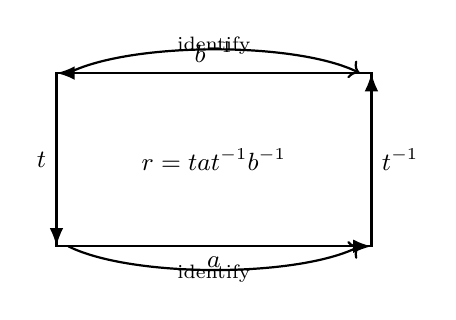
\begin{tikzpicture}[scale=1]
% Draw as a rectangle with left/right identified (standard annulus cut)
\coordinate (A) at (0,0);
\coordinate (B) at (4,0);
\coordinate (C) at (4,2.2);
\coordinate (D) at (0,2.2);
\draw[face] (A)--(B)--(C)--(D)--cycle;

% boundary labels (a cyclic shift of t a t^{-1} b^{-1})
\draw[edge] (A)-- node[below]{$a$} (B);
\draw[edge] (B)-- node[right]{$t^{-1}$} (C);
\draw[edge] (C)-- node[above]{$b^{-1}$} (D);
\draw[edge] (D)-- node[left]{$t$} (A);

\node at (2,1.1) {$r=t a t^{-1}b^{-1}$};

% indicate identification of left and right sides (annulus gluing)
\draw[->,thick] ($(D)+(0.15,0)$) .. controls +(0.8,0.4) and +(-0.8,0.4) .. ($(C)+(-0.15,0)$);
\draw[->,thick] ($(A)+(0.15,0)$) .. controls +(0.8,-0.4) and +(-0.8,-0.4) .. ($(B)+(-0.15,0)$);
\node at (2,2.55) {\scriptsize identify};
\node at (2,-0.35) {\scriptsize identify};
\end{tikzpicture}
\caption{Cut-open annular diagram: gluing the $t$-side to the $t^{-1}$-side yields an annulus with boundary cycles labeled by $a$ and $b$.}
\end{figure}
\clearpage
% ============================================================
\section{van Kampen diagram}

\subsection*{Definition}
Over $\mathcal P=\langle X\mid R\rangle$, a \emph{van Kampen diagram} for a word $w\in (X^{\pm1})^*$ is a disk diagram $D\to K(\mathcal P)$
such that each 2-cell boundary label is a cyclic conjugate of some $r\in R^{\pm1}$, and the outer boundary label is $w$.

\subsection*{Existence/uniqueness (precise statement)}
\begin{theorem}[van Kampen's lemma + normal closure interpretation]\label{thm:vK}
Let $\mathcal P=\langle X\mid R\rangle$ and let $w$ be a word in $X^{\pm1}$.
\begin{enumerate}[leftmargin=2.2em]
\item (\textbf{Existence equivalence}) $w=1$ in $G(\mathcal P)$ if and only if there exists a van Kampen disk diagram over $\mathcal P$ with boundary label $w$.
\item (\textbf{Normal closure equivalence}) Equivalently, $w$ lies in the normal closure of $R$ in $F(X)$:
\[
w\in \langle\!\langle R\rangle\!\rangle \quad\Longleftrightarrow\quad
w=\prod_{i=1}^N u_i r_i^{\varepsilon_i}u_i^{-1}\text{ in }F(X).
\]
\item (\textbf{Minimal area exists}) If $w=1$ in $G(\mathcal P)$, then among all van Kampen diagrams for $w$ there exists one with minimal area (fewest 2-cells).
\item (\textbf{Non-uniqueness}) Van Kampen diagrams for the same boundary word are generally not unique up to isomorphism, even among minimal-area diagrams.
\end{enumerate}
\end{theorem}


\paragraph{Non-uniqueness: in what sense?}
Even if you fix the \emph{based} boundary cycle and the \emph{exact linear} word $w$ (not just its cyclic rotation),
there can be many non-isomorphic van Kampen diagrams with boundary label $w$.
Operations that preserve the boundary word but change the diagram include:
\begin{itemize}[leftmargin=2em]
\item inserting/removing cancellable dipoles (a pair of adjacent faces labeled by $r$ and $r^{-1}$ sharing an edge-path),
\item different planar gluings realizing the same product-of-conjugates proof,
\item different reduced/minimal-area fillings (minimal area itself is an invariant, but minimizers need not be unique).
\end{itemize}
So ``unique up to isomorphism'' does \emph{not} hold for van Kampen diagrams; what is canonical is the \emph{existence} equivalence and often the \emph{minimal area value}.
\subsection*{Algorithm A (Forward): product of conjugates $\to$ van Kampen diagram (very detailed)}\cite{vanKampen1933,lyndonschupp1977}
\paragraph{Input.} A representation in the free group
\[
w=\prod_{i=1}^N u_i r_i^{\varepsilon_i}u_i^{-1},
\quad r_i\in R,\;\varepsilon_i=\pm 1.
\]
\paragraph{Output.} A planar simply connected labeled 2-complex with boundary label $w$.

\paragraph{Steps.}
\begin{enumerate}[leftmargin=2.2em]
\item \textbf{Create faces.}
For each $i$, draw a polygonal 2-cell $f_i$ whose boundary cycle is subdivided and oriented so that reading around it gives a cyclic conjugate of $r_i^{\varepsilon_i}$.

\item \textbf{Choose attachment points.}
On each face boundary $\partial f_i$, choose a distinguished vertex $p_i$ (a ``pin'').

\item \textbf{Attach whiskers for conjugation.}
Create a new basepoint vertex $*$ on the outside.
For each $i$, attach a path $P_i$ from $*$ to $p_i$ whose label is $u_i$.
(So traversing $P_i$ then $\partial f_i$ then $P_i^{-1}$ reads $u_i r_i^{\varepsilon_i}u_i^{-1}$.)

\item \textbf{Form a boundary word and glue cancellations.}
Consider the big loop based at $*$ that runs:
\[
P_1\,\partial f_1\,P_1^{-1}\; P_2\,\partial f_2\,P_2^{-1}\;\cdots\; P_N\,\partial f_N\,P_N^{-1}.
\]
Its label is exactly the product $\prod u_i r_i^{\varepsilon_i}u_i^{-1}$, which freely reduces to $w$.

Now perform \emph{edge identifications} corresponding to free cancellations:
whenever the concatenation of these loops produces adjacent letters $a a^{-1}$, identify the corresponding two boundary edges (with opposite orientations).
Continue until all cancellations are realized.

\item \textbf{Extract the outer boundary.}
After all identifications, the remaining unglued boundary cycle is the outer boundary $\partial D$ and its label is $w$.

\item \textbf{Optional simplification: remove spurs/dipoles.}
If the resulting complex contains immediate cancellable face pairs (dipoles) or boundary spurs, cancel them to obtain a reduced diagram.
\end{enumerate}

\paragraph{Boundary cases.}
\begin{itemize}[leftmargin=2em]
\item \textbf{Empty boundary word.} If $w$ freely reduces to $\varepsilon$, then the empty diagram (no faces) certifies $w=1$.
\item \textbf{Single relator.} If $w$ is (a cyclic conjugate of) $r^{\pm1}$ for some $r\in R$, then one 2-cell suffices.
\end{itemize}

\paragraph{Complexity (rough).}\cite{vanKampen1933,lyndonschupp1977}
Assume the input is a product-of-conjugates proof with total length
\[
L_{\mathrm{proof}} := |w| + \sum_{i=1}^N \bigl(2|u_i|+|r_i|\bigr).
\]
\begin{itemize}[leftmargin=2em]
\item Creating the faces and whiskers costs $O(L_{\mathrm{proof}})$ time and space.
\item Gluing all free cancellations can be implemented in near-linear time in the boundary size using union-find / hashing,
but a safe bound for a naive implementation is $O(L_{\mathrm{proof}}^2)$ time.
\item The size of the resulting diagram is $O(L_{\mathrm{proof}})$ cells/edges/vertices (before optional reductions).
\end{itemize}


\subsection*{Algorithm B (Inverse): van Kampen diagram $\to$ product of conjugates (very detailed)}\cite{vanKampen1933,lyndonschupp1977}
\paragraph{Input.} A van Kampen diagram $D$ over $\mathcal P$ with boundary label $w$.
\paragraph{Output.} An explicit equality $w=\prod u_f r_f^{\varepsilon_f}u_f^{-1}$ in $F(X)$.

\paragraph{Steps.}
\begin{enumerate}[leftmargin=2.2em]
\item Choose a basepoint $*\in\partial D$ on the outer boundary.
\item Choose a spanning tree $T$ in $D^{(1)}$ containing all boundary vertices.
\item For each face $f\in \Faces(D)$:
\begin{enumerate}[leftmargin=2em]
\item pick a boundary vertex $p_f\in\partial f$,
\item let $u_f=\lab(\text{tree path in }T\text{ from }*\text{ to }p_f)$,
\item read the face boundary label starting at $p_f$ (consistent orientation) to obtain a cyclic conjugate of some relator $r_f^{\varepsilon_f}$.
\end{enumerate}
\item Then in the free group,
\[
w=\prod_{f\in \Faces(D)} u_f\, r_f^{\varepsilon_f}\, u_f^{-1},
\]
where the product order can be taken by traversing faces in any order consistent with a planar reduction (e.g.\ peel faces one-by-one from the boundary).
\end{enumerate}



\paragraph{Boundary cases and choices.}
\begin{itemize}[leftmargin=2em]
\item If $D$ has no faces, then $w$ must be freely trivial and the extracted product is empty.
\item Different spanning trees produce different conjugator words $u_f$, but all yield valid certificates of the same equality in $F(X)$.
\end{itemize}

\paragraph{Complexity (rough).}\cite{lyndonschupp1977}
Let $D$ have $(|V|,|E|,|F|)$ and total perimeter $P$.
\begin{itemize}[leftmargin=2em]
\item Build a spanning tree: $O(|V|+|E|)$ time.
\item Read all face boundary labels: $O(P)$ time.
\item Total extraction time: $O(|V|+|E|+P)$, with space $O(|V|+|E|)$.
\end{itemize}
\subsection*{Worked example: one-face van Kampen diagram for $[a,b]$}
This is the same as the commutator disk: $w=aba^{-1}b^{-1}$ is itself a relator.

\paragraph{Forward (Algorithm A).}
\begin{enumerate}[leftmargin=2.2em]
\item Write $w=u_1 r_1 u_1^{-1}$ with $u_1=\varepsilon$ and $r_1=w$.
\item Create one square face labeled by $w$; no gluing is required.
\end{enumerate}

\paragraph{Inverse (Algorithm B).}
\begin{enumerate}[leftmargin=2.2em]
\item Choose basepoint on boundary; choose a spanning tree of the 1-skeleton.
\item There is one face $f$ with $u_f=\varepsilon$ and $r_f=w$.
\item Output $w=\varepsilon\cdot w\cdot \varepsilon^{-1}$.
\end{enumerate}

\begin{figure}[h]
\centering
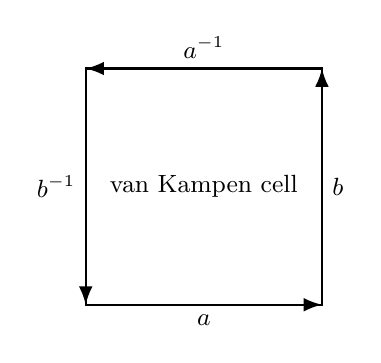
\begin{tikzpicture}[scale=1]
\coordinate (A) at (0,0);
\coordinate (B) at (3,0);
\coordinate (C) at (3,3);
\coordinate (D) at (0,3);
\draw[face] (A)--(B)--(C)--(D)--cycle;
\draw[edge] (A) -- node[below]{$a$} (B);
\draw[edge] (B) -- node[right]{$b$} (C);
\draw[edge] (C) -- node[above]{$a^{-1}$} (D);
\draw[edge] (D) -- node[left]{$b^{-1}$} (A);
\node at (1.5,1.5) {\small van Kampen cell};
\end{tikzpicture}
\caption{A one-face van Kampen diagram for $w=aba^{-1}b^{-1}$.}
\end{figure}
\clearpage
% ============================================================
\section{Dehn diagram}

\subsection*{Definition}
In a reduced van Kampen disk diagram $D$, a face $f$ is a \emph{Dehn cell} if
$\partial f$ shares a \emph{contiguous} arc with the outer boundary $\partial D$ of length \emph{strictly more than half} the perimeter of $f$.
A \emph{Dehn diagram} is a van Kampen disk diagram viewed through this ``peeling'' lens.

\subsection*{Existence/uniqueness (concrete theorem)}
\begin{theorem}[Greendlinger-type Dehn cell existence under $C'(1/6)$]\label{thm:greendlinger}
Let $\mathcal P=\langle X\mid R\rangle$ be a (classical) small-cancellation presentation satisfying $C'(1/6)$.
Then every nontrivial reduced van Kampen disk diagram $D$ over $\mathcal P$ contains a Dehn cell:
there exists a face $f$ such that $\partial f$ shares with $\partial D$ a contiguous boundary subpath of length $>\tfrac12|\partial f|$.
In particular, any nontrivial null-homotopic word admits a Dehn-reduction step that strictly shortens the boundary length.
\end{theorem}

\begin{remark}
Other standard hypotheses also guarantee Dehn cells (e.g.\ $C'(1/4)$--$T(4)$ and $C'(1/3)$--$T(6)$).
We state $C'(1/6)$ for concreteness.
\end{remark}

\subsection*{Algorithm A (Forward): Dehn reductions $\to$ a peeling diagram (detailed)}\cite{dehn1911,greendlinger1960,lyndonschupp1977}
\paragraph{Input.}
A word $w$ and a sequence of Dehn reductions
\[
w=w_0\to w_1\to\cdots\to w_k=\varepsilon
\]
where each step replaces a subword longer than half a relator by the complementary shorter subword.

\paragraph{Output.} A van Kampen disk diagram whose faces correspond to the reduction steps.

\paragraph{Steps.}
\begin{enumerate}[leftmargin=2.2em]
\item Initialize a polygonal boundary cycle subdivided into $|w_0|$ directed edges labeled by $w_0$.
This is the boundary of a ``current partial diagram'' with no faces.
\item For each reduction step $w_{i-1}\to w_i$:
\begin{enumerate}[leftmargin=2em]
\item Choose a relator $r\in R^{\pm1}$ and a cyclic decomposition $r=uv$ such that $u$ occurs as a contiguous subword of the current boundary word
and $|u|>\tfrac12|r|$.
\item Glue a new 2-cell labeled by $r$ to the current diagram by identifying the $u$-arc of $\partial r$ with the $u$-arc on the outer boundary.
\item After gluing, the complementary arc $v$ becomes part of the new outer boundary.
\item Freely reduce the new outer boundary word; this reduced word is $w_i$.
\end{enumerate}
\item After $k$ steps, the boundary word is empty; the result is a disk diagram for $w$.
By construction each added face is a Dehn cell at the moment it is added.
\end{enumerate}


\paragraph{Boundary cases.}
\begin{itemize}[leftmargin=2em]
\item If the reduction sequence has length $k=0$ (so $w=\varepsilon$), then the output diagram is the empty diagram.
\item If a reduction step uses $u=\partial r$ (gluing along the entire boundary), then that step adds a face and immediately removes that boundary component.
\end{itemize}

\paragraph{Complexity (rough).}\cite{dehn1911,greendlinger1960,lyndonschupp1977}
Let $n_i=|w_i|$ and let $F=k$ be the number of Dehn reduction steps (so also the number of faces created).
\begin{itemize}[leftmargin=2em]
\item Building the initial boundary and gluing one face per step takes time proportional to the total boundary work performed.
A safe bound is $O\!\left(\sum_{i=0}^{k-1} n_i\right)$ for a combinatorial implementation where each step edits the boundary cyclic word.
\item In the worst case $n_i$ decreases by only $1$ each step, so $\sum n_i=O(n_0^2)$, giving a simple bound $O(n_0^2)$ time.
\end{itemize}

\subsection*{Algorithm B (Inverse): peel a Dehn diagram to produce reductions (detailed)}\cite{dehn1911,greendlinger1960,lyndonschupp1977}
\paragraph{Input.} A reduced van Kampen disk diagram $D$ over a presentation satisfying the Dehn cell property.
\paragraph{Output.} A sequence of Dehn reductions reducing the boundary word to empty.

\paragraph{Steps.}
\begin{enumerate}[leftmargin=2.2em]
\item Let $w_0$ be the boundary word of $D$.
\item While $D$ has at least one face:
\begin{enumerate}[leftmargin=2em]
\item Find a Dehn cell $f$ (guaranteed by Theorem~\ref{thm:greendlinger} under $C'(1/6)$).
\item Let $u$ be the long boundary arc of $\partial f$ that lies on the outer boundary $\partial D$; let $v$ be the complementary arc of $\partial f$.
\item Remove $f$ from the diagram and replace the boundary segment $u$ by $v$.
\item Freely reduce the resulting boundary word; call it $w_{i+1}$.
\end{enumerate}
\item Output the sequence $w_0\to w_1\to\cdots\to \varepsilon$.
Each step strictly decreases length.
\end{enumerate}



\paragraph{Boundary cases and implementation notes.}
\begin{itemize}[leftmargin=2em]
\item If $D$ has no faces, the boundary word is already freely trivial and the output reduction sequence is length $0$.
\item Finding a Dehn cell is the only nontrivial step. Under $C'(1/6)$ (or similar hypotheses), a Dehn cell exists in any nontrivial reduced diagram, so the loop terminates.
\end{itemize}

\paragraph{Complexity (rough).}\cite{lyndonschupp1977}
Let $D$ have $F$ faces and total perimeter $P$.
\begin{itemize}[leftmargin=2em]
\item \textbf{Peeling a \emph{given} diagram.} A naive implementation that scans all faces to find a Dehn cell at each peel step costs $O(P)$ per step, hence $O(PF)$ time in the worst case.
With suitable bookkeeping of boundary adjacency, one can do better, but $O(PF)$ is a safe bound.
\item \textbf{Dehn's word reduction algorithm (word-only view).} If you implement Dehn reduction by repeatedly scanning the current word of length $\le n$ for a ``long'' subword of some relator, a simple bound is $O(n^2\|R\|)$ time (at most $n$ reductions, each scan costs $O(n\|R\|)$).
\end{itemize}
\subsection*{Worked example: $\langle a\mid a^6\rangle$ and $w=a^6$}
This example is small and illustrates the peeling idea concretely.

\paragraph{Forward (Algorithm A).}
\begin{enumerate}[leftmargin=2.2em]
\item Presentation has one relator $r=a^6$.
\item Start with boundary cycle labeled $w_0=a^6$ (a 6-gon boundary).
\item Glue one 2-cell labeled $a^6$ along the entire boundary word $u=a^6$.
Here $|u|=6>\tfrac12\cdot 6=3$, so it is (trivially) a Dehn attachment.
\item After gluing, no boundary remains: $w_1=\varepsilon$.
\end{enumerate}

\paragraph{Inverse (Algorithm B).}
\begin{enumerate}[leftmargin=2.2em]
\item The diagram has exactly one face and its entire boundary lies on $\partial D$, so it is a Dehn cell.
\item Peel it off: boundary becomes empty in one step.
\end{enumerate}

\begin{figure}[h]
\centering
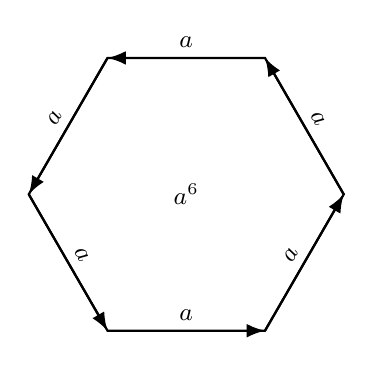
\begin{tikzpicture}[scale=1]
\foreach \k in {0,...,5} {
  \coordinate (P\k) at ({2*cos(60*\k)},{2*sin(60*\k)});
}
\draw[face] (P0)--(P1)--(P2)--(P3)--(P4)--(P5)--cycle;
\foreach \k/\knext in {0/1,1/2,2/3,3/4,4/5,5/0} {
  \draw[edge] (P\k) -- node[midway,sloped,above]{$a$} (P\knext);
}
\node at (0,0) {$a^6$};
\end{tikzpicture}
\caption{A Dehn diagram for $a^6$ with one hexagonal Dehn cell.}
\end{figure}
\clearpage
% ============================================================
\section{Spherical diagram}

\subsection*{Definition}
A \emph{spherical diagram} over $\mathcal P$ is a finite labeled 2-complex $S\to K(\mathcal P)$ whose underlying space is the sphere $S^2$ (no boundary).
A spherical diagram is \emph{reduced} if it contains no \emph{dipole} (a cancellable adjacent pair of faces with inverse labels along a common edge-path).

\subsection*{Existence/uniqueness (precise statement)}
\begin{theorem}[Spherical diagrams, $\pi_2$, and identities among relators]\label{thm:spherical}
Let $\mathcal P=\langle X\mid R\rangle$.
\begin{enumerate}[leftmargin=2.2em]
\item (\textbf{Existence} $\Leftrightarrow \pi_2$) There exists a nontrivial reduced spherical diagram over $\mathcal P$
if and only if $\pi_2(K(\mathcal P))\neq 0$.
\item (\textbf{Algebraic meaning}) A spherical diagram determines an \emph{identity among relators}:
\[
\prod_{i=1}^N u_i\, r_i^{\varepsilon_i}\,u_i^{-1}=1 \quad\text{in }F(X),
\]
and conversely such an identity can be realized by a spherical diagram (after gluing cancellations).
\item (\textbf{Non-uniqueness}) Spherical diagrams are not unique; many non-isomorphic diagrams can represent the same element of $\pi_2$.
\end{enumerate}
\end{theorem}

\subsection*{Algorithm A (Forward): identity among relators $\to$ spherical diagram (detailed)}\cite{gersten1987,lyndonschupp1977}
\paragraph{Input.} An identity in the free group:
\[
\prod_{i=1}^N u_i\, r_i^{\varepsilon_i}\,u_i^{-1}=1.
\]
\paragraph{Output.} A closed labeled surface diagram (a sphere in the simplest case).

\paragraph{Steps.}
\begin{enumerate}[leftmargin=2.2em]
\item For each $i$, create a face $f_i$ labeled by $r_i^{\varepsilon_i}$ and choose a pin vertex $p_i\in\partial f_i$.
\item Create a basepoint $*$ and attach a whisker path $P_i$ from $*$ to $p_i$ labeled by $u_i$.
\item Consider the boundary word of the concatenation of loops $P_i\,\partial f_i\,P_i^{-1}$.
Because the product equals $1$, this word freely reduces to the empty word.
\item Perform edge identifications for each cancellation until no boundary remains.
\item The resulting closed diagram is (typically) a sphere; in general the gluing might produce another closed surface.
When it is $S^2$, you have a spherical diagram.


\paragraph{Boundary cases.}
\begin{itemize}[leftmargin=2em]
\item The empty identity (no factors) gives the empty diagram (no faces). A \emph{nontrivial} spherical diagram requires at least one face.
\item The construction may yield a closed surface of genus $>0$ if the identifications do not produce $S^2$. Spherical diagrams are the genus-$0$ case.
\end{itemize}

\paragraph{Complexity (rough).}\cite{gersten1987,sieradski1983,lyndonschupp1977}
Let the identity have total length
\[
L_{\mathrm{id}} := \sum_{i=1}^N \bigl(2|u_i|+|r_i|\bigr).
\]
\begin{itemize}[leftmargin=2em]
\item Building faces and whiskers costs $O(L_{\mathrm{id}})$ time/space.
\item Performing all cancellation gluings costs at most quadratic time $O(L_{\mathrm{id}}^2)$ in a naive implementation; near-linear is possible with union-find, but $O(L_{\mathrm{id}}^2)$ is a safe bound.
\end{itemize}
\end{enumerate}

\subsection*{Algorithm B (Inverse): spherical diagram $\to$ identity among relators (detailed)}\cite{gersten1987,lyndonschupp1977}
\paragraph{Input.} A spherical diagram $S$ over $\mathcal P$.
\paragraph{Output.} An identity among relators.

\paragraph{Steps.}
\begin{enumerate}[leftmargin=2.2em]
\item Choose a basepoint vertex $*\in S^{(1)}$ and a spanning tree $T\subseteq S^{(1)}$.
\item For each face $f$:
\begin{enumerate}[leftmargin=2em]
\item choose a boundary vertex $p_f\in\partial f$,
\item let $u_f=\lab(\text{tree path }*\to p_f)$,
\item read the relator word $r_f^{\varepsilon_f}$ around $\partial f$ starting at $p_f$.
\end{enumerate}
\item Multiply the conjugates $u_f r_f^{\varepsilon_f}u_f^{-1}$ over all faces.
Because $S$ has no boundary, the product equals $1$ in $F(X)$.
\end{enumerate}



\paragraph{Complexity (rough).}\cite{gersten1987}
Let $S$ have $(|V|,|E|,|F|)$ and total perimeter $P=\sum_f|\partial f|$.
\begin{itemize}[leftmargin=2em]
\item Building a spanning tree: $O(|V|+|E|)$.
\item Reading all face boundaries: $O(P)$.
\item Total extraction time: $O(|V|+|E|+P)$ with space $O(|V|+|E|)$.
\end{itemize}
\subsection*{Worked example: two-face dipole sphere ($r\cdot r^{-1}=1$)}
\paragraph{Forward (Algorithm A).}
\begin{enumerate}[leftmargin=2.2em]
\item Start with the identity $r\cdot r^{-1}=1$.
\item Create two faces: $f_1$ labeled $r$ and $f_2$ labeled $r^{-1}$.
\item Glue their entire boundaries edge-by-edge (matching labels with opposite orientations).
\item The result is a sphere with two faces: a dipole.
\end{enumerate}

\paragraph{Inverse (Algorithm B).}
\begin{enumerate}[leftmargin=2.2em]
\item Choose basepoint and spanning tree.
\item Each face contributes a conjugate of $r$ or $r^{-1}$.
\item The extracted identity is (up to trivial conjugations) $r\cdot r^{-1}=1$.
\end{enumerate}

\begin{figure}[h]
\centering
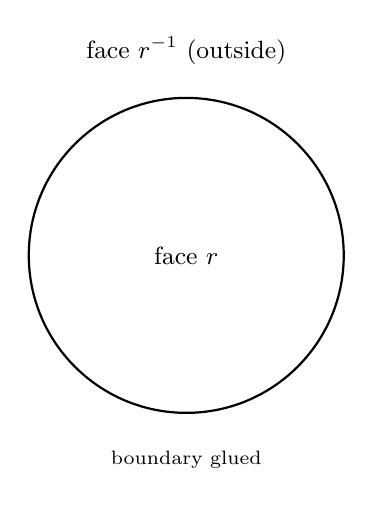
\begin{tikzpicture}[scale=1]
% Represent sphere as disk + exterior region: a circle separating two faces.
\draw[face] (0,0) circle (2);
\node at (0,0) {face $r$};
\node at (0,2.6) {face $r^{-1}$ (outside)};
\node at (0,-2.6) {\scriptsize boundary glued};
\end{tikzpicture}
\caption{Planar depiction of a spherical diagram: interior region labeled $r$ and the exterior region labeled $r^{-1}$.}
\end{figure}
\clearpage
% ============================================================
\section{Howie diagram (relative diagrams)}

\subsection*{Definition (detailed)}
Let $G$ be a base group and let
\[
\mathcal P_{\mathrm{rel}}=\langle G, X \mid \mathcal R\rangle
\]
be a \emph{relative presentation}, where relators lie in the free product $G*F(X)$.
Write a relator in alternating form:
\[
r=g_0 x_1 g_1 x_2 \cdots x_n g_n,\quad g_i\in G,\ x_i\in X^{\pm1}.
\]

A \emph{Howie diagram} (one standard convention) is a disk or sphere diagram where:
\begin{itemize}[leftmargin=2em]
\item oriented edges are labeled by letters of $X^{\pm1}$,
\item \emph{corners} (angles between consecutive edges along a face) are labeled by elements of $G$,
\item reading around each face (alternating corner labels and edge labels) yields a cyclic conjugate of some $r\in\mathcal R^{\pm1}$,
\item around each vertex, the product of corner labels (in cyclic order) equals $1$ in $G$.
\end{itemize}

\subsection*{Existence/uniqueness (precise statement)}
\begin{theorem}[Relative van Kampen / Howie lemma]\label{thm:howie}
Let $\mathcal P_{\mathrm{rel}}=\langle G,X\mid \mathcal R\rangle$ and let $W$ be an alternating boundary word in $G*F(X)$.
Then
\[
W=1 \text{ in } \langle G,X\mid \mathcal R\rangle
\quad\Longleftrightarrow\quad
\text{there exists a Howie disk diagram over }\mathcal P_{\mathrm{rel}}\text{ with boundary }W.
\]
Howie diagrams are generally not unique for fixed boundary data.
\end{theorem}


\paragraph{Non-uniqueness (what can vary).}
Even with the boundary word $W$ fixed as an element of the free product $G*F(X)$ (not just up to cyclic rotation),
Howie diagrams are generally not unique: different planar gluings, insertion/removal of dipoles, and different choices of spanning tree/basepoint
produce non-isomorphic diagrams encoding the same equality.
\subsection*{Algorithm A (Forward): relative equality $\to$ Howie diagram (detailed)}
\paragraph{Input.}
An explicit identity in the free product $G*F(X)$ of the form
\[
W=\prod_{i=1}^N U_i\, R_i^{\varepsilon_i}\,U_i^{-1},
\]
where each $R_i\in \mathcal R$ is a relator word and $U_i\in G*F(X)$.

\paragraph{Output.} A Howie disk diagram with boundary $W$.

\paragraph{Steps.}
\begin{enumerate}[leftmargin=2.2em]
\item Write each relator $R_i$ in alternating form $g_0 x_1 g_1 \cdots x_n g_n$.
\item For each relator occurrence, create a face:
\begin{itemize}[leftmargin=2em]
\item put the $x_j$ on directed edges in cyclic order,
\item put the $g_j$ on corners between edges.
\end{itemize}
\item Attach ``whiskers'' (paths in the edge-labeled 1-skeleton) encoding the conjugators $U_i$.
\item Glue boundary edges labeled by $X^{\pm1}$ according to cancellations in the product.
\item The vertex corner-label condition (product equals $1$ in $G$) is automatically satisfied if the algebraic identity holds;
combinatorially, it ensures the diagram consistently records coefficients in $G$.


\paragraph{Boundary cases.}
\begin{itemize}[leftmargin=2em]
\item If $W=\varepsilon$ and $N=0$, the output is the empty diagram.
\item If there is a single relator factor (and $U_1=\varepsilon$), the diagram has one face.
\end{itemize}

\paragraph{Complexity (rough).}\cite{howie1981,howie1984}
Let
\[
L_{\mathrm{rel}} := \sum_{i=1}^N \bigl(2|U_i|+|R_i|\bigr),
\]
where lengths are measured in the alternating normal form in $G*F(X)$ (counting $X$-letters and recording $G$-coefficients).
\begin{itemize}[leftmargin=2em]
\item Creating faces and whiskers costs $O(L_{\mathrm{rel}})$ time/space.
\item Performing all cancellation gluings among $X$-edges costs at most $O(L_{\mathrm{rel}}^2)$ time in a naive implementation.
\end{itemize}
\end{enumerate}

\subsection*{Algorithm B (Inverse): Howie diagram $\to$ relative equality (detailed)}
\paragraph{Input.} A Howie disk diagram $D$ with boundary word $W$.
\paragraph{Output.} A derivation showing $W=1$ in the relative group.

\paragraph{Steps.}
\begin{enumerate}[leftmargin=2.2em]
\item Choose a basepoint on the boundary and a spanning tree $T$ in the edge-labeled 1-skeleton.
\item For each face $f$:
\begin{enumerate}[leftmargin=2em]
\item choose a boundary corner/vertex on $\partial f$,
\item read the alternating face word $R_f^{\varepsilon_f}$ (corners in $G$, edges in $X^{\pm1}$),
\item compute the conjugator $U_f$ as the word in $G*F(X)$ obtained by reading the tree path from the basepoint to that chosen place.
\end{enumerate}
\item Multiply the conjugates $\prod_f U_f R_f^{\varepsilon_f}U_f^{-1}$; it equals $W$ (disk case) or $1$ (sphere case).
\end{enumerate}



\paragraph{Complexity (rough).}\cite{howie1981,howie1984}
Let $D$ have $(|V|,|E|,|F|)$ and let $P$ be the total number of $X$-labeled edge occurrences around all faces (the ``$X$-perimeter'').
\begin{itemize}[leftmargin=2em]
\item Build a spanning tree: $O(|V|+|E|)$.
\item Read all face boundary data: $O(P)$ to read $X$-edges plus the cost of multiplying/recording corner labels in $G$ (treated here as $O(1)$ per corner if group operations in $G$ are $O(1)$).
\item Total extraction time: $O(|V|+|E|+P)$.
\end{itemize}
\subsection*{Worked example: $\langle G,t \mid t^{-1} a t b^{-1}\rangle$}
Fix $a,b\in G$ and consider the relative presentation with one relator $t^{-1} a t b^{-1}$.

\paragraph{Forward (Algorithm A).}
\begin{enumerate}[leftmargin=2.2em]
\item Here $X=\{t\}$ and $\mathcal R=\{t^{-1} a t b^{-1}\}$.
\item Create one face. Its boundary alternates:
edge $t^{-1}$, corner $a$, edge $t$, corner $b^{-1}$.
\item The boundary word of the diagram is $t^{-1} a t b^{-1}$, hence it is trivial in the quotient.
\end{enumerate}

\paragraph{Inverse (Algorithm B).}
\begin{enumerate}[leftmargin=2.2em]
\item Read the unique face boundary word $t^{-1} a t b^{-1}$.
\item Conclude $t^{-1} a t b^{-1}=1$ in the relative group, hence $t^{-1} a t=b$.
\end{enumerate}

\begin{figure}[h]
\centering
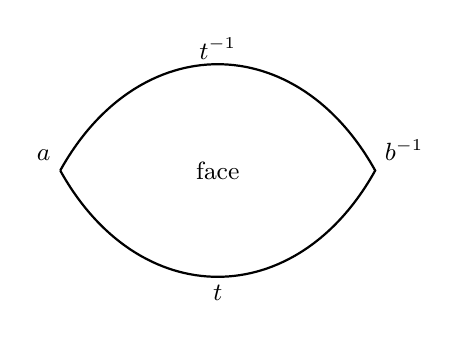
\begin{tikzpicture}[scale=1]
% Draw a "bigon" with two edge labels and two corner labels
\coordinate (L) at (-2,0);
\coordinate (R) at (2,0);
\draw[face] (L) .. controls (-1,1.8) and (1,1.8) .. (R)
            .. controls (1,-1.8) and (-1,-1.8) .. (L);
% edge labels
\node at (0,1.55) {$t^{-1}$};
\node at (0,-1.55) {$t$};
% corner labels
\node[above left] at (L) {$a$};
\node[above right] at (R) {$b^{-1}$};
\node at (0,0) {face};
\end{tikzpicture}
\caption{A one-face Howie diagram encoding the relative relator $t^{-1} a t b^{-1}$. Edges are labeled by $t^{\pm1}$ and corners by elements of $G$.}
\end{figure}

% ============================================================
\section{Aspherical diagram (asphericity via absence of reduced spheres)}

\subsection*{Definition}
A 2-complex $X$ is \emph{aspherical} if $\pi_2(X)=0$.
For a presentation $\mathcal P$, we say $\mathcal P$ is aspherical if the presentation complex $K(\mathcal P)$ is aspherical.

\subsection*{Existence/uniqueness (property theorem, detailed)}
\begin{theorem}[Asphericity and spherical diagrams]\label{thm:aspherical}
Let $\mathcal P=\langle X\mid R\rangle$.
The following are equivalent:
\begin{enumerate}[leftmargin=2.2em]
\item $K(\mathcal P)$ is aspherical: $\pi_2(K(\mathcal P))=0$.
\item There exists \emph{no} nontrivial reduced spherical diagram over $\mathcal P$.
\item Every spherical diagram over $\mathcal P$ can be reduced to the empty diagram by cancelling dipoles.
\end{enumerate}
Moreover, a stronger sufficient condition is \emph{diagrammatic reducibility (DR)}:
every spherical diagram contains a dipole. DR implies asphericity.
\end{theorem}


\paragraph{Algorithmic remark (complexity for a \emph{given} spherical diagram).}
If you are handed a specific spherical diagram $S$, then you can attempt to reduce it by cancelling dipoles:
\begin{itemize}[leftmargin=2em]
\item A single dipole cancellation can be found by scanning adjacent face pairs along shared edges; a naive scan costs $O(P)$ where $P$ is total perimeter.
\item Each cancellation strictly decreases the number of faces, so at most $|F|$ cancellations occur.
Thus a safe bound for reducing a \emph{given} diagram is $O(P|F|)$ time.
\end{itemize}
\textbf{Warning.} Theorem~\ref{thm:aspherical} is a characterization, but deciding whether an arbitrary finite presentation is aspherical is a subtle global problem;
in general one should not expect a simple efficient algorithm without additional hypotheses (small cancellation, CAT(0) cube complex structure, etc.).
\subsection*{Example 1: free group wedge of circles is aspherical}
\paragraph{Forward construction (space viewpoint).}
\begin{enumerate}[leftmargin=2.2em]
\item The presentation complex $K(\langle a,b\mid\ \rangle)$ has one vertex and two 1-cells, with no 2-cells.
So $K$ is a graph (1-dimensional CW complex).
\item Any 2-sphere map into a 1-dimensional complex is null-homotopic, hence $\pi_2(K)=0$.
\end{enumerate}

\paragraph{Inverse diagram viewpoint.}
\begin{enumerate}[leftmargin=2.2em]
\item A spherical diagram would require faces labeled by relators.
\item There are no relators and no 2-cells, so no spherical diagrams exist.
\end{enumerate}

\begin{figure}[h]
\centering
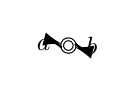
\begin{tikzpicture}[scale=1]
\node[basevtx] (v) at (0,0) {};
\draw[edge,loop left] (v) to node[left]{$a$} (v);
\draw[edge,loop right] (v) to node[right]{$b$} (v);
\end{tikzpicture}
\caption{A wedge of two circles: the presentation complex for $\langle a,b\mid\ \rangle\cong F_2$.}
\end{figure}

\subsection*{Example 2: the torus presentation $\langle a,b\mid [a,b]\rangle$ is aspherical}
\paragraph{Forward (universal cover viewpoint).}
\begin{enumerate}[leftmargin=2.2em]
\item The Cayley graph of $\langle a,b\mid [a,b]\rangle$ is the square grid.
\item Attach a square 2-cell to every unit square cycle in the grid (each labeled by the commutator).
\item The resulting simply connected 2-complex is the square tiling of the plane $\mathbb R^2$, which is contractible.
\item Therefore the universal cover of $K(\mathcal P)$ is contractible, implying $\pi_2(K(\mathcal P))=0$.
\end{enumerate}

\paragraph{Inverse (diagram obstruction viewpoint).}
\begin{enumerate}[leftmargin=2.2em]
\item If a reduced spherical diagram existed, it would represent a nontrivial element of $\pi_2(K(\mathcal P))$.
\item Lifting to the contractible universal cover would make it null-homotopic, contradiction.
\item Hence no reduced spherical diagrams exist, consistent with Theorem~\ref{thm:aspherical}.
\end{enumerate}

\begin{figure}[h]
\centering
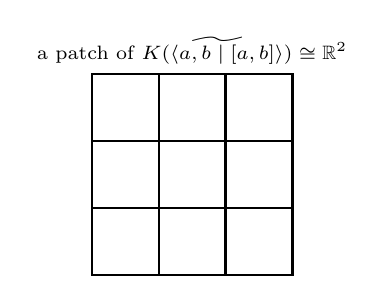
\begin{tikzpicture}[scale=0.85]
% draw a 3x3 tiling patch
\foreach \i in {0,1,2} {
  \foreach \j in {0,1,2} {
    \draw[thick] (\i,\j) rectangle (\i+1,\j+1);
  }
}
\node at (1.5,3.35) {\scriptsize a patch of $\widetilde{K(\langle a,b\mid [a,b]\rangle)}\cong \mathbb R^2$};
\end{tikzpicture}
\caption{A finite patch of the square tiling universal cover of the torus presentation complex.}
\end{figure}

% ============================================================
\section{Triangle diagram}

\subsection*{Definition}
A \emph{triangle diagram} is a van Kampen diagram in which every face is a triangle (3-gon).
This is natural for \emph{triangular presentations} where every relator has length $3$.

\subsection*{Existence/uniqueness (detailed)}
\begin{proposition}[Triangle diagrams: existence and relation to general diagrams]\label{prop:triangle}
\begin{enumerate}[leftmargin=2.2em]
\item If $\mathcal P=\langle X\mid R\rangle$ is triangular (every $r\in R$ has length $3$),
then every van Kampen diagram over $\mathcal P$ is automatically a triangle diagram.

\item More generally, any polygonal disk diagram can be subdivided into triangles
(e.g.\ by barycentric subdivision of the 2-complex $D$).
This changes the cell structure of the diagram but not the boundary word it fills.
\end{enumerate}
Triangle diagrams are generally not unique.
\end{proposition}

\subsection*{Algorithm A (Forward): build a triangle diagram (detailed)}\cite{hatcher2002}
\paragraph{Input.}
Either:
\begin{itemize}[leftmargin=2em]
\item a triangular presentation and a proof of triviality $w=1$ (as a product of conjugates), or
\item a general polygonal van Kampen diagram to be triangulated.
\end{itemize}

\paragraph{Output.}
A triangle diagram.

\paragraph{Steps (triangular presentation).}
\begin{enumerate}[leftmargin=2.2em]
\item Express $w=\prod u_i r_i^{\varepsilon_i}u_i^{-1}$ where each $r_i$ has length $3$.
\item Apply van Kampen Algorithm A: each face $r_i^{\varepsilon_i}$ is drawn as a triangle.
\item Glue cancellations; all faces remain triangles.
\end{enumerate}

\paragraph{Steps (triangulating a polygonal diagram).}
\begin{enumerate}[leftmargin=2.2em]
\item For each $n$-gon face, insert a new vertex at its center and connect it to all boundary vertices (barycentric subdivision).
\item This subdivides the face into $n$ triangles.
\item Repeat for all faces; keep all existing edge labels on original edges.
New edges are ``auxiliary'' edges in the subdivided diagram (in topology they map into $X$ by the cellular map).


\paragraph{Boundary cases.}
\begin{itemize}[leftmargin=2em]
\item If the input diagram already has only triangular faces, the triangulation procedure does nothing.
\item If $n=3$, you may choose to leave the triangular face as-is (do nothing). If you apply the coning (star) subdivision anyway, it splits into 3 triangles. If you instead apply true barycentric subdivision, it splits into 6 triangles.
\end{itemize}

\paragraph{Complexity (rough).}\cite{hatcher2002}
\begin{itemize}[leftmargin=2em]
\item \textbf{From a triangular presentation + proof.} Same as van Kampen Algorithm~A: if the proof has total length $L_{\mathrm{proof}}$, then a safe bound is $O(L_{\mathrm{proof}}^2)$ time for naive gluing and $O(L_{\mathrm{proof}})$ space.
\item \textbf{Triangulating an existing polygonal diagram.} Let $P=\sum_f |\partial f|$ be the total perimeter.
Barycentric subdivision adds exactly $|\partial f|$ triangles in each face $f$, so the new number of faces is $O(P)$.
The subdivision can be performed in $O(P)$ time and produces $O(P)$ new edges/vertices.
\end{itemize}
\end{enumerate}

\subsection*{Algorithm B (Inverse): triangle diagram $\to$ relator product (detailed)}\cite{hatcher2002}
\paragraph{Input.} A triangle diagram $D$ over a presentation $\mathcal P=\langle X\mid R\rangle$ (so each face boundary is a cyclic conjugate of some $r\in R^{\pm1}$ and has length $3$).
\paragraph{Output.} An explicit equality in the free group
\[
w=\prod_{f\in \Faces(D)} u_f\, r_f^{\varepsilon_f}\,u_f^{-1},
\]
where $w$ is the outer boundary word of $D$.

\paragraph{Steps.}
\begin{enumerate}[leftmargin=2.2em]
\item Choose a basepoint $*\in \partial D$ on the outer boundary.
\item Choose a spanning tree $T$ in the 1-skeleton $D^{(1)}$ containing all boundary vertices.
\item For each triangular face $f$:
\begin{enumerate}[leftmargin=2em]
\item choose a vertex $p_f$ on $\partial f$,
\item define $u_f=\lab(\text{the unique path in }T\text{ from }*\text{ to }p_f)$,
\item read the (length $3$) cyclic word around $\partial f$ starting at $p_f$ to obtain a cyclic conjugate of a relator $r_f^{\varepsilon_f}$.
\end{enumerate}
\item Multiply the conjugates in any order obtained by peeling faces from the boundary (so that the product corresponds to the cancellation of internal edges).
The resulting product equals the boundary word $w$ in $F(X)$.
\end{enumerate}



\paragraph{Complexity (rough).}\cite{hatcher2002}
If $D$ has $(|V|,|E|,|F|)$ and total perimeter $P$, then extracting a relator product by choosing a spanning tree and reading each triangular face costs
$O(|V|+|E|+P)$ time and $O(|V|+|E|)$ space, as in the van Kampen case.
\subsection*{Worked example: $\langle a,b,c\mid abc\rangle$}
\paragraph{Forward (triangular presentation).}
\begin{enumerate}[leftmargin=2.2em]
\item Relator $r=abc$ has length $3$.
\item Boundary word $w=abc$.
\item Build one triangular face with boundary labels $a,b,c$.
\end{enumerate}

\paragraph{Inverse .}
\begin{enumerate}[leftmargin=2.2em]
\item Choose basepoint on boundary.
\item There is one face and the conjugator is trivial; hence $w=r$.
\end{enumerate}

\begin{figure}[h]
\centering
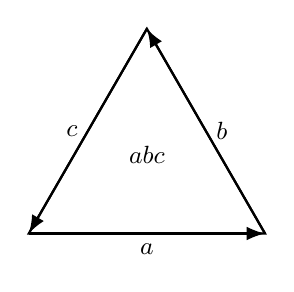
\begin{tikzpicture}[scale=1]
\coordinate (A) at (0,0);
\coordinate (B) at (3,0);
\coordinate (C) at (1.5,2.6);
\draw[face] (A)--(B)--(C)--cycle;
\draw[edge] (A)-- node[below]{$a$} (B);
\draw[edge] (B)-- node[right]{$b$} (C);
\draw[edge] (C)-- node[left]{$c$} (A);
\node at (1.5,1.0) {$abc$};
\end{tikzpicture}
\caption{A one-face triangle diagram for the relator $abc$.}
\end{figure}

% ============================================================
\section{Polygonal complex}

\subsection*{Definition}
A \emph{polygonal complex} is a 2-dimensional CW-complex whose 2-cells are polygons attached along edge cycles.

\subsection*{Existence/uniqueness (detailed theorem)}
\begin{theorem}[Presentation complexes and reconstruction]\label{thm:poly}
\begin{enumerate}[leftmargin=2.2em]
\item (\textbf{Existence}) For every presentation $\mathcal P=\langle X\mid R\rangle$ there exists a polygonal 2-complex $K(\mathcal P)$ (the presentation complex)
with $\pi_1(K(\mathcal P))\cong G(\mathcal P)$.

\item (\textbf{Uniqueness with fixed combinatorics}) If the cyclic representative of each relator and the orientations/labels of the generator loops are fixed,
then $K(\mathcal P)$ is unique up to a label-preserving cellular isomorphism.

\item (\textbf{Reconstruction}) Conversely, for any connected polygonal complex $X$ there is a standard algorithm to extract a presentation for $\pi_1(X)$:
choose a maximal tree in the 1-skeleton, make generators from non-tree edges, and relators from 2-cell attaching maps.
Different tree choices yield Tietze-equivalent presentations.
\end{enumerate}
\end{theorem}

\subsection*{Algorithm A (Forward): presentation $\to K(\mathcal P)$ (detailed)}\cite{hatcher2002,bridsonhaefliger1999}
\paragraph{Input.} $\mathcal P=\langle X\mid R\rangle$.
\paragraph{Output.} A labeled polygonal complex $K(\mathcal P)$.

\paragraph{Steps.}
\begin{enumerate}[leftmargin=2.2em]
\item Create one vertex $v_0$.
\item For each generator $x\in X$, attach an oriented loop edge at $v_0$ labeled $x$.
\item For each relator $r=a_1\cdots a_n$ with $a_i\in X^{\pm1}$:
\begin{enumerate}[leftmargin=2em]
\item create an $n$-gon 2-cell $f_r$ whose boundary is subdivided into $n$ directed edges,
\item label these boundary edges in order by $a_1,\dots,a_n$,
\item glue the boundary to the 1-skeleton by mapping each labeled edge to the corresponding generator loop (with orientation determined by $a_i$).
\end{enumerate}
\item The resulting CW-complex is $K(\mathcal P)$.


\paragraph{Boundary cases.}
\begin{itemize}[leftmargin=2em]
\item \textbf{No relators.} If $R=\varnothing$, then $K(\mathcal P)$ is a wedge of $|X|$ circles (a 1-dimensional CW-complex).
\item \textbf{Trivial group.} If $X=\varnothing$ and $R=\varnothing$, then $K(\mathcal P)$ is a single point and $\pi_1$ is trivial.
\end{itemize}

\paragraph{Complexity (rough).}\cite{hatcher2002,bridsonhaefliger1999}
Let $\|R\|=\sum_{r\in R}|r|$.
\begin{itemize}[leftmargin=2em]
\item Building the 1-skeleton takes $O(|X|)$ time and space.
\item Creating and attaching all 2-cells takes $O(\|R\|)$ time and produces $O(\|R\|)$ boundary edge occurrences.
\item Total size of $K(\mathcal P)$ is $O(|X|+\|R\|)$ cells, so the forward construction is linear in the input size.
\end{itemize}
\end{enumerate}

\subsection*{Algorithm B (Inverse): polygonal complex $\to$ a presentation for $\pi_1$ (detailed)}\cite{hatcher2002,bridsonhaefliger1999}
\paragraph{Input.} A connected polygonal complex $X$.
\paragraph{Output.} A presentation for $\pi_1(X)$.

\paragraph{Steps.}
\begin{enumerate}[leftmargin=2.2em]
\item Choose a maximal spanning tree $T$ in the 1-skeleton $X^{(1)}$.
\item For each oriented edge $e$ of $X^{(1)}$ not in $T$, introduce a generator $x_e$ (and identify $x_{\overline e}=x_e^{-1}$).
\item For each 2-cell $f$:
\begin{enumerate}[leftmargin=2em]
\item traverse its attaching cycle once around, recording a word in the generators:
when you traverse a non-tree edge $e$, write $x_e$ (or $x_e^{-1}$ if traversed backwards);
when you traverse a tree edge, write nothing (tree edges become trivial in the quotient).
\item The resulting word is a relator $r_f$.
\end{enumerate}
\item Output the presentation
\[
\pi_1(X)\cong \langle x_e\ (e\notin T)\mid r_f\ (f\in X^{(2)})\rangle .
\]
\end{enumerate}



\paragraph{Complexity (rough).}\cite{hatcher2002,bridsonhaefliger1999}
Let $X$ have $|V|$ vertices and $|E|$ edges in its 1-skeleton, and let $P=\sum_f|\partial f|$ be total perimeter of 2-cells.
\begin{itemize}[leftmargin=2em]
\item Spanning tree computation: $O(|V|+|E|)$ time.
\item Reading all 2-cell attaching cycles: $O(P)$ time.
\item Total extraction time: $O(|V|+|E|+P)$, with output size proportional to the number of non-tree edges and the total relator length you read.
\end{itemize}
\subsection*{Worked example: fundamental polygon for the torus}
\paragraph{Forward (Algorithm A).}
\begin{enumerate}[leftmargin=2.2em]
\item Presentation: $\langle a,b\mid aba^{-1}b^{-1}\rangle$.
\item 1-skeleton: one vertex, two loop edges labeled $a$ and $b$.
\item Attach one square 2-cell whose boundary is labeled $a,b,a^{-1},b^{-1}$.
\item The resulting complex is a 2-torus (a polygonal complex with one square face).
\end{enumerate}

\paragraph{Inverse (Algorithm B).}
\begin{enumerate}[leftmargin=2.2em]
\item Choose maximal tree $T$ to be just the vertex (no edges).
Then both loop edges are non-tree edges: generators are $a$ and $b$.
\item The square face boundary reads $aba^{-1}b^{-1}$, giving the relator.
\item Hence $\pi_1\cong \langle a,b\mid aba^{-1}b^{-1}\rangle$.
\end{enumerate}

\begin{figure}[h]
\centering
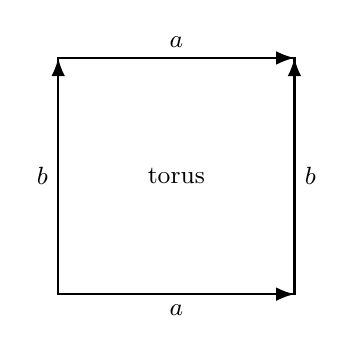
\begin{tikzpicture}[scale=1]
\coordinate (A) at (0,0);
\coordinate (B) at (3,0);
\coordinate (C) at (3,3);
\coordinate (D) at (0,3);
\draw[face] (A)--(B)--(C)--(D)--cycle;
% arrows on edges indicating identifications/orientations
\draw[edge] (A)-- node[below]{$a$} (B);
\draw[edge] (D)-- node[above]{$a$} (C);
\draw[edge] (A)-- node[left]{$b$} (D);
\draw[edge] (B)-- node[right]{$b$} (C);
\node at (1.5,1.5) {\small torus};
\end{tikzpicture}
\caption{A square fundamental polygon for the torus (a polygonal complex with one square 2-cell).}
\end{figure}

% ============================================================
\section{RAAG diagram (Salvetti / cube complex)}

\subsection*{Definition}
Given a finite simplicial graph $\Gamma$, the right-angled Artin group (RAAG) is
\[
A_\Gamma=\langle V(\Gamma)\mid [v,w]=1 \text{ whenever }\{v,w\}\in E(\Gamma)\rangle.
\]
The \emph{Salvetti complex} $S_\Gamma$ is the canonical cube complex built from $\Gamma$:
one loop per generator, one square per commuting pair, and higher-dimensional cubes for cliques.

\subsection*{Existence/uniqueness (detailed theorem)}
\begin{theorem}[Salvetti complex: existence, uniqueness, and reconstruction]\label{thm:salvetti}
Let $\Gamma$ be a finite simplicial graph and $A_\Gamma$ its RAAG.
\begin{enumerate}[leftmargin=2.2em]
\item (\textbf{Existence}) There exists a cube complex $S_\Gamma$ such that $\pi_1(S_\Gamma)\cong A_\Gamma$.
\item (\textbf{Asphericity}) $S_\Gamma$ is a $K(A_\Gamma,1)$: its universal cover $\widetilde{S_\Gamma}$ is contractible (indeed CAT(0)).
\item (\textbf{Uniqueness}) The cubical isomorphism class of $S_\Gamma$ is uniquely determined by $\Gamma$.
\item (\textbf{Reconstruction of $\Gamma$}) The graph $\Gamma$ can be recovered from $S_\Gamma$:
its vertices correspond to 1-cells at the unique vertex of $S_\Gamma$, and two vertices are adjacent in $\Gamma$
iff the corresponding 1-cells span a square 2-cell in $S_\Gamma$ (equivalently: they commute in $\pi_1$).
\end{enumerate}
\end{theorem}

\subsection*{Algorithm A (Forward): $\Gamma\to S_\Gamma$ (detailed)}\cite{green1990,salvetti1987,charney2007,bridsonhaefliger1999,gromov1987}
\paragraph{Input.} A finite simplicial graph $\Gamma$.
\paragraph{Output.} The cube complex $S_\Gamma$.

\paragraph{Steps.}
\begin{enumerate}[leftmargin=2.2em]
\item Create one vertex $v_0$.
\item For each vertex $x\in V(\Gamma)$, attach a loop edge at $v_0$ labeled $x$.
\item For each edge $\{x,y\}\in E(\Gamma)$, attach a square 2-cell whose boundary is labeled $xyx^{-1}y^{-1}$.
This enforces the commutation relation $[x,y]=1$.
\item For each clique $C=\{x_1,\dots,x_k\}$ (complete subgraph):
attach a $k$-cube whose 1-skeleton uses the loop edges labeled $x_i$ and whose 2-faces are exactly the commuting squares from the edges in $C$.
(Equivalently: attach a $k$-torus cell structure for the abelian subgroup $\langle C\rangle\cong\mathbb Z^k$.)


\paragraph{Boundary cases.}
\begin{itemize}[leftmargin=2em]
\item \textbf{Empty graph.} If $V(\Gamma)=\varnothing$, then $A_\Gamma$ is trivial and $S_\Gamma$ is a single vertex (a point).
\item \textbf{Complete graph.} If $\Gamma$ is complete on $n$ vertices, then $A_\Gamma\cong \mathbb Z^n$ and $S_\Gamma$ is an $n$-torus cellulation (one $k$-cube for each $k$-subset).
\end{itemize}

\paragraph{Complexity (rough).}\cite{salvetti1987,charney2007,bridsonhaefliger1999,gromov1987}
Let $n=|V(\Gamma)|$ and $m=|E(\Gamma)|$.
\begin{itemize}[leftmargin=2em]
\item Building the \textbf{1-skeleton} takes $O(n)$ time and space.
\item Building the \textbf{2-skeleton} (adding one square per edge) takes $O(m)$ time and adds $m$ squares.
\item Building the \textbf{full Salvetti complex} requires adding a $k$-cube for every clique of size $k$.
The number of cliques can be exponential in $n$ in the worst case, so constructing the entire complex is exponential in general.
(For many applications one works only up to some fixed dimension, e.g.\ the 2-skeleton.)
\end{itemize}
\end{enumerate}

\subsection*{Algorithm B (Inverse): $S_\Gamma\to \Gamma$ and the RAAG presentation (detailed)}\cite{green1990,salvetti1987,charney2007,bridsonhaefliger1999,gromov1987}
\paragraph{Input.} A Salvetti-type cube complex $S$ with one vertex.
\paragraph{Output.} The defining graph $\Gamma$ and the RAAG presentation.

\paragraph{Steps.}
\begin{enumerate}[leftmargin=2.2em]
\item List the oriented 1-cells (loops) at the unique vertex; call their labels $V$.
These are the generators.
\item For each unordered pair $\{x,y\}\subseteq V$, check if there is a square 2-cell whose boundary word is $xyx^{-1}y^{-1}$.
If yes, put an edge between $x$ and $y$.
\item The resulting graph is $\Gamma$ and the recovered group presentation is
\[
\langle V \mid [x,y]=1 \text{ for each edge }\{x,y\}\in E(\Gamma)\rangle.
\]
\end{enumerate}



\paragraph{Complexity (rough).}\cite{salvetti1987,charney2007}
Suppose $S$ has one vertex, $n$ loop 1-cells, and $q$ square 2-cells.
\begin{itemize}[leftmargin=2em]
\item Listing the generators (1-cells) costs $O(n)$.
\item Checking commutations by scanning the list of squares costs $O(q)$ if the squares are stored with their edge labels.
A naive pairwise check over all unordered pairs of generators is $O(n^2)$, but in practice $q$ is the relevant parameter.
\item Output size: $n$ generators and $q$ commutator relations.
\end{itemize}
\subsection*{Example 1: no edge $\Rightarrow A_\Gamma\cong F_2$}
\paragraph{Forward (Algorithm A).}
\begin{enumerate}[leftmargin=2.2em]
\item $\Gamma$ has vertices $\{a,b\}$ and no edge.
\item Build $S_\Gamma$:
one vertex and two loop edges labeled $a$ and $b$.
\item There are no edges in $\Gamma$, hence attach no squares and no higher cubes.
\item Therefore $\pi_1(S_\Gamma)\cong \langle a,b\mid\ \rangle\cong F_2$.
\end{enumerate}

\paragraph{Inverse (Algorithm B).}
\begin{enumerate}[leftmargin=2.2em]
\item From $S_\Gamma$, generators are the two 1-cells $a$ and $b$.
\item There is no square 2-cell, so no commuting relations.
\item Hence recovered $\Gamma$ has no edge and recovered group is $F_2$.
\end{enumerate}

\begin{figure}[h]
\centering
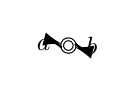
\begin{tikzpicture}[scale=1]
\node[basevtx] (v) at (0,0) {};
\draw[edge,loop left] (v) to node[left]{$a$} (v);
\draw[edge,loop right] (v) to node[right]{$b$} (v);
\end{tikzpicture}
\caption{Salvetti complex for $\Gamma$ with two isolated vertices: a wedge of two circles, $\pi_1\cong F_2$.}
\end{figure}

\subsection*{Example 2: one edge $\Rightarrow A_\Gamma\cong \mathbb Z^2$}
\paragraph{Forward (Algorithm A).}
\begin{enumerate}[leftmargin=2.2em]
\item $\Gamma$ has vertices $\{a,b\}$ with a single edge $\{a,b\}$.
\item Build 1-skeleton: one vertex with loops labeled $a$ and $b$.
\item Because $\{a,b\}$ is an edge, attach one square with boundary word $aba^{-1}b^{-1}$.
\item No higher cubes exist (no 3-cliques), so the result is a 2-torus cell structure.
Thus $\pi_1\cong \langle a,b\mid [a,b]\rangle\cong \mathbb Z^2$.
\end{enumerate}

\paragraph{Inverse (Algorithm B).}
\begin{enumerate}[leftmargin=2.2em]
\item Generators are the two 1-cells $a$ and $b$.
\item There is a square with commutator boundary, hence $a$ and $b$ commute and $\{a,b\}$ is an edge in $\Gamma$.
\item Therefore recovered $\Gamma$ is an edge graph and the recovered group is $\mathbb Z^2$.
\end{enumerate}

\begin{figure}[h]
\centering
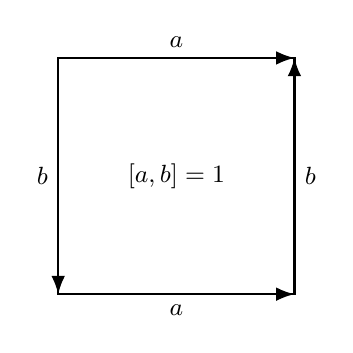
\begin{tikzpicture}[scale=1]
\coordinate (A) at (0,0);
\coordinate (B) at (3,0);
\coordinate (C) at (3,3);
\coordinate (D) at (0,3);
\draw[face] (A)--(B)--(C)--(D)--cycle;
\draw[edge] (A)-- node[below]{$a$} (B);
\draw[edge] (B)-- node[right]{$b$} (C);
\draw[edge] (D)-- node[left]{$b$} (A);
\draw[edge] (D)-- node[above]{$a$} (C);
\node at (1.5,1.5) {$[a,b]=1$};
\end{tikzpicture}
\caption{Salvetti complex for an edge graph on $\{a,b\}$: a square 2-cell yields $\mathbb Z^2$.}
\end{figure}

\clearpage
% ============================================================
\section{Automatic group diagram (automatic structures)}

\subsection*{Definition}
Fix a finitely generated group $G=\langle A\rangle$ with a finite \emph{symmetric} generating set $A=A^{-1}$.
An \emph{automatic structure} for the marked group $(G,A)$ consists of:
\begin{itemize}[leftmargin=2em]
\item a regular language $L\subseteq A^*$ (the \emph{combing language}) such that the evaluation map
$\pi:A^*\to G$ is surjective on $L$ (every $g\in G$ has at least one representative in $L$);
\item for each $a\in A\cup\{1\}$, a finite automaton recognizing the \emph{multiplier relation}
\[
R_a \;=\;\{(u,v)\in L\times L:\ \pi(u)\,a=\pi(v)\ \text{in }G\},
\]
viewed as a \emph{synchronous} regular language over a padded product alphabet (see below).
\end{itemize}
The resulting ``diagram'' is the package of automata: a \emph{word-acceptor} for $L$ and \emph{multiplier automata} for $R_a$.

\subsection*{Synchronous padding (the input format for multiplier diagrams)}
Let $\$ \notin A$ be a padding symbol and let $\widehat A:=A\cup\{\$\}$.
Define a padding map
\[
\mathrm{pad}:A^*\times A^*\longrightarrow (\widehat A\times \widehat A)^*
\]
by aligning two words letter-by-letter and padding the shorter one with $\$$.
Formally, if $u=u_1\cdots u_m$ and $v=v_1\cdots v_n$ and $\ell=\max\{m,n\}$, then
\[
\mathrm{pad}(u,v)_i=
\begin{cases}
(u_i,v_i) & i\le m,\ i\le n,\\
(u_i,\$)  & i\le m,\ i>n,\\
(\$,v_i)  & i>m,\ i\le n.
\end{cases}
\]
We identify $R_a$ with the language $\{\mathrm{pad}(u,v):(u,v)\in R_a\}\subseteq(\widehat A\times\widehat A)^*$.
A \emph{multiplier diagram} is the directed labeled graph of a finite automaton over alphabet $(\widehat A\times\widehat A)$
accepting this padded language.

\subsection*{Existence/uniqueness (precise statement)}
\begin{theorem}[Automatic structures: invariance and what is (not) canonical]\label{thm:automatic-structure}
Let $G$ be a finitely generated group.
\begin{enumerate}[leftmargin=2.2em]
\item (\textbf{Existence as a property}) The statement ``$G$ is automatic'' means: for some (equivalently any) finite symmetric generating set $A$,
there exists an automatic structure $(L,\{R_a\}_{a\in A\cup\{1\}})$ for $(G,A)$.

\item (\textbf{Non-uniqueness of structure}) Even for fixed $(G,A)$, the choice of $L$ and the multiplier automata is generally \emph{not} unique.
Different regular combings can encode the same group.

\item (\textbf{Uniqueness of recognized relations}) Once $(G,A)$ and $L$ are fixed,
each relation $R_a\subseteq L\times L$ is determined uniquely as a set.
Hence the \emph{minimal} deterministic finite automaton recognizing the padded language of $R_a$
is unique up to isomorphism of labeled directed graphs.

\item (\textbf{Reconstruction of multiplication on normal forms}) If $L$ gives \emph{unique} normal forms (i.e.\ $\pi|_L$ is bijective),
then the family $\{R_a\}$ uniquely determines the right-multiplication action of $A$ on $G$ written in normal form.
\end{enumerate}
\end{theorem}

\subsection*{Algorithm A (Forward): build the automatic-group diagram}
\paragraph{Input.}
A finitely generated group $G=\langle A\rangle$ together with:
\begin{itemize}[leftmargin=2em]
\item a specification of a regular combing language $L\subseteq A^*$ (ideally by an automaton);
\item a method to decide/compute, for each $u\in L$ and $a\in A\cup\{1\}$, some $v\in L$ with $\pi(u)a=\pi(v)$
(e.g.\ a known normal-form procedure, or a known automatic structure from theory).
\end{itemize}

\paragraph{Output.}
A \emph{word-acceptor} automaton for $L$ and multiplier automata for the padded relations $R_a$.

\paragraph{Steps (conceptual).}
\begin{enumerate}[leftmargin=2.2em]
\item Construct (or record) a DFA/NFA $\mathcal A_L$ recognizing $L$.
\item For each $a\in A\cup\{1\}$, define the relation
$R_a=\{(u,v)\in L\times L:\pi(u)a=\pi(v)\}$.
\item Build a finite automaton $\mathcal M_a$ recognizing the padded language
$\{\mathrm{pad}(u,v):(u,v)\in R_a\}\subseteq(\widehat A\times\widehat A)^*$.
\item Output the package $(\mathcal A_L,\{\mathcal M_a\}_{a\in A\cup\{1\}})$ as the automatic-group diagram.
\end{enumerate}

\paragraph{Boundary cases and implementation notes.}
\begin{itemize}[leftmargin=2em]
\item \textbf{Surjectivity vs.\ uniqueness.} The definition only requires $L\twoheadrightarrow G$.
If you enforce uniqueness (normal forms), Algorithm~B becomes cleaner but may require extra work to compute $v\in L$ uniquely.
\item \textbf{Padding symbol.} The padding symbol $\$$ is \emph{not} a generator; it exists only to align pairs $(u,v)$.
\item \textbf{Identity multiplier.} The case $a=1$ should recognize equality within $L$: $R_1=\{(u,u):u\in L\}$.
\end{itemize}

\paragraph{Complexity (rough).}
Let $N_L$ be the number of states of the automaton for $L$ and let $N_a$ be the number of states in $\mathcal M_a$.
\begin{itemize}[leftmargin=2em]
\item \textbf{Membership in $L$.} Testing $w\in L$ by running $\mathcal A_L$ takes $O(|w|)$ time.
\item \textbf{Checking a multiplier relation.} Given $u,v\in L$, testing whether $(u,v)\in R_a$ by running $\mathcal M_a$ on $\mathrm{pad}(u,v)$
takes $O(\max\{|u|,|v|\})$ time.
\item \textbf{Building automata.} If $\mathcal A_L$ and $\mathcal M_a$ are given explicitly, producing the diagram is linear in their descriptions
(e.g.\ $O(N_L+ \sum_a N_a)$ to store).
Constructing $\mathcal M_a$ \emph{from scratch} depends on the chosen normal-form machinery and is the main nontrivial cost in practice.
\end{itemize}

\subsection*{Algorithm B (Inverse / use): solve the word problem using the automatic diagram}
\paragraph{Input.}
A word-acceptor $\mathcal A_L$ for $L$ and multiplier automata $\{\mathcal M_a\}_{a\in A\cup\{1\}}$
for an automatic structure on $(G,A)$.

\paragraph{Output.}
A procedure to decide whether two input words represent the same element of $G$ (word problem);
optionally, a normal-form representative in $L$ when $L$ is unique.

\paragraph{Steps (standard ``multiplier chase'').}
\begin{enumerate}[leftmargin=2.2em]
\item (Optional) If inputs are already in $L$, skip to Step~3. Otherwise choose representatives in $L$ for the inputs.
When $L$ is a unique normal form language, compute/approximate the $L$-representative by multiplying the identity normal form
by letters of the input word and repeatedly applying multipliers (see Step~3).
\item Given words $w_1,w_2\in A^*$, reduce the problem to comparing elements in $L$:
find $u,v\in L$ with $\pi(u)=\pi(w_1)$ and $\pi(v)=\pi(w_2)$.
\item To multiply an $L$-word $u$ by a generator $a\in A$, find $v\in L$ with $(u,v)\in R_a$.
Operationally, this means: search for an accepting run of $\mathcal M_a$ on some padded pair $(u,v)$.
(If $L$ is unique and $\mathcal M_a$ is deterministic and functional, this $v$ is unique.)
\item Decide whether $w_1=_G w_2$ by checking whether the obtained $u$ and $v$ are equal as words in $L$ (or whether $(u,v)\in R_1$).
\end{enumerate}

\paragraph{Complexity (rough).}
\begin{itemize}[leftmargin=2em]
\item If inputs are already in $L$, checking equality via $R_1$ is $O(|u|)$.
\item Converting an arbitrary word of length $n$ to an $L$-representative by iterated multiplication uses $n$ multiplier steps.
In the best-case ``functional deterministic'' setting, this is often near $O(n)$ in practice;
in the worst case, maintaining and updating representatives can lead to $O(n^2)$ total time (depending on the structure and bookkeeping).
\end{itemize}

\subsection*{Worked example: $G=\mathbb Z$ with a regular combing and one multiplier}
Take $A=\{t,t^{-1}\}$ and the regular language of \emph{signed normal forms}
\[
L \;=\; \{t^n:n\ge 0\}\ \cup\ \{(t^{-1})^n:n\ge 1\}\ \cup\ \{\varepsilon\}.
\]
(So $0$ is represented by $\varepsilon$; positives by $t^n$; negatives by $(t^{-1})^n$.)

\paragraph{Word-acceptor (for $L$).}
It accepts $\varepsilon$, any string of only $t$'s, or any string of only $t^{-1}$'s, but rejects mixed-sign words.

\begin{figure}[h]
\centering
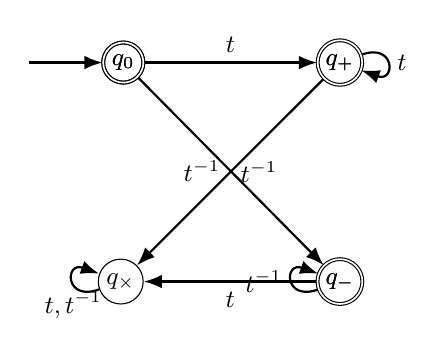
\begin{tikzpicture}[node distance=22mm]
\node[basevtx] (q0) {$q_0$};
\node[vtx, right=of q0] (qp) {$q_+$};
\node[vtx, below=of qp] (qm) {$q_-$};
\node[vtx, left=of qm] (qd) {$q_\times$};

% start arrow
\draw[edge] ($(q0)+(-1.2,0)$) -- (q0);

% transitions
\draw[edge] (q0) -- node[above] {$t$} (qp);
\draw[edge] (q0) -- node[left] {$t^{-1}$} (qm);
\draw[edge] (qp) to[out=20,in=340,looseness=6] node[right] {$t$} (qp);
\draw[edge] (qm) to[out=200,in=160,looseness=6] node[left] {$t^{-1}$} (qm);

% reject sink for mixed signs (schematic)
\draw[edge] (qp) -- node[right] {$t^{-1}$} (qd);
\draw[edge] (qm) -- node[below] {$t$} (qd);
\draw[edge] (qd) to[out=200,in=160,looseness=6] node[below] {$t,t^{-1}$} (qd);

% accepting indication (use double border as a visual cue)
\node[basevtx] at (q0) {$q_0$};
\node[basevtx] at (qp) {$q_+$};
\node[basevtx] at (qm) {$q_-$};
\end{tikzpicture}
\caption{A schematic word-acceptor for $L\subseteq\{t,t^{-1}\}^*$. (Here double circles indicate accepting states.)}
\end{figure}

\paragraph{Multiplier diagram for right-multiplication by $t$ (sketch).}
The relation $R_t$ consists of pairs $(u,v)\in L\times L$ with $\pi(u)t=\pi(v)$.
Concretely:
\begin{itemize}[leftmargin=2em]
\item if $u=t^k$ then $v=t^{k+1}$;
\item if $u=(t^{-1})$ then $v=\varepsilon$;
\item if $u=(t^{-1})^k$ with $k\ge 2$ then $v=(t^{-1})^{k-1}$.
\end{itemize}
A finite automaton over the padded alphabet $(\widehat A\times\widehat A)$ can recognize these cases.
(For a fully explicit minimal diagram, you would list its states and transitions case-by-case; this is where you insert your preferred level of detail.)
% ------------------------------------------------------------



% ============================================================
\section{Automaton group automaton (Mealy automata and tree actions)}

\subsection*{Definition}
A (deterministic) \emph{Mealy automaton} is a quadruple
\[
\mathcal M=(Q,\Sigma,\delta,\lambda),
\]
where $Q$ is a finite set of states, $\Sigma$ is a finite input alphabet,
\[
\delta:Q\times\Sigma\to Q \quad\text{(transition)},\qquad
\lambda:Q\times\Sigma\to \Sigma \quad\text{(output)}.
\]
We draw an edge
\[
q \xrightarrow{\ a\mid b\ } \delta(q,a)
\qquad\text{whenever } \lambda(q,a)=b.
\]
The automaton is \emph{invertible} if for every $q\in Q$ the map $a\mapsto \lambda(q,a)$ is a permutation of $\Sigma$.

\subsection*{Existence/uniqueness (precise statement)}
\begin{theorem}[From an invertible Mealy automaton to a group of tree automorphisms]\label{thm:mealy-to-group}
Let $\mathcal M=(Q,\Sigma,\delta,\lambda)$ be a Mealy automaton.
\begin{enumerate}[leftmargin=2.2em]
\item (\textbf{Existence}) Each state $q\in Q$ defines a unique length-preserving map
$f_q:\Sigma^*\to\Sigma^*$ by the recursion
\[
f_q(\varepsilon)=\varepsilon,\qquad
f_q(a w)=\lambda(q,a)\, f_{\delta(q,a)}(w)\quad (a\in\Sigma,\ w\in\Sigma^*).
\]

\item (\textbf{Uniqueness}) The action $f_q$ is uniquely determined by the labeled directed graph of $\mathcal M$
(i.e.\ by the transition/output data).

\item (\textbf{Group case}) If $\mathcal M$ is invertible, then each $f_q$ is a rooted tree automorphism of the regular rooted tree $T_\Sigma$
(with vertex set $\Sigma^*$), hence $f_q\in\mathrm{Aut}(T_\Sigma)$, and the subgroup
\[
G(\mathcal M):=\langle f_q:q\in Q\rangle \le \mathrm{Aut}(T_\Sigma)
\]
is called the \emph{automaton group} generated by $\mathcal M$.

\item (\textbf{Reconstruction criterion}) Conversely, if you are given a set of tree automorphisms described by wreath recursions
whose set of \emph{sections} is finite and closed under taking sections, then one can reconstruct an equivalent finite Mealy automaton
producing the same action (Algorithm~B below).
\end{enumerate}
\end{theorem}

\subsection*{Algorithm A (Forward): build the automaton-group diagram and induced action}
\paragraph{Input.}
An invertible Mealy automaton $\mathcal M=(Q,\Sigma,\delta,\lambda)$.

\paragraph{Output.}
The Mealy diagram (state graph with labels $a\mid b$), and an oracle for the induced maps $f_q:\Sigma^*\to\Sigma^*$.

\paragraph{Steps.}
\begin{enumerate}[leftmargin=2.2em]
\item \textbf{Verify invertibility.} For each $q\in Q$, check that $a\mapsto \lambda(q,a)$ is a permutation of $\Sigma$.
\item \textbf{Record the diagram.} Draw the directed labeled graph with edges $q\xrightarrow{a\mid \lambda(q,a)}\delta(q,a)$.
\item \textbf{Define the action.} For any word $w\in\Sigma^*$ and state $q\in Q$, compute $f_q(w)$ by the recursion
$f_q(a w)=\lambda(q,a)\, f_{\delta(q,a)}(w)$.
\item \textbf{Output the group.} The automaton group is $G(\mathcal M)=\langle f_q:q\in Q\rangle$ (given by generators-as-states).
\end{enumerate}

\paragraph{Boundary cases and implementation notes.}
\begin{itemize}[leftmargin=2em]
\item \textbf{Non-invertible automata.} If invertibility fails, each $f_q$ is still a tree \emph{endomorphism} but may not be invertible,
so you do not obtain a subgroup of $\mathrm{Aut}(T_\Sigma)$.
\item \textbf{Minimization.} As with DFAs, Mealy automata can often be minimized (merge equivalent states), changing the diagram but not the induced action.
\end{itemize}

\paragraph{Complexity (rough).}
Let $m=|Q|$ and $k=|\Sigma|$.
\begin{itemize}[leftmargin=2em]
\item \textbf{Invertibility test.} $O(mk)$ time by scanning outputs per state (e.g.\ counting occurrences).
\item \textbf{Apply a state to an input word.} Computing $f_q(w)$ for $|w|=n$ takes $O(n)$ time.
\item \textbf{Level-$n$ Schreier graph (optional).} The action on $\Sigma^n$ has $k^n$ vertices.
Building the labeled Schreier graph for $r$ chosen generators costs $O(r\cdot k^n \cdot n)$ time if you compute each image by $O(n)$ recursion.
\end{itemize}

\subsection*{Algorithm B (Inverse): reconstruct a Mealy automaton from finite wreath recursion}
\paragraph{Input.}
A finite alphabet $\Sigma$ and a finite set of generators acting on $T_\Sigma$ given in \emph{wreath recursion} form:
\[
g \equiv (g|_a)_{a\in\Sigma}\ \pi_g,
\]
where $\pi_g\in\mathrm{Sym}(\Sigma)$ is the first-letter permutation and each $g|_a$ (the \emph{section at $a$}) is again one of finitely many states.
Assume the set of all states you see is finite and closed under taking sections.

\paragraph{Output.}
A finite invertible Mealy automaton $\mathcal M=(Q,\Sigma,\delta,\lambda)$ producing the same tree action.

\paragraph{Steps.}
\begin{enumerate}[leftmargin=2.2em]
\item \textbf{State set.} Let $Q$ be the finite closure of the given generators under taking sections $g\mapsto g|_a$ for all $a\in\Sigma$.
\item \textbf{Output function.} For each $q\in Q$ and $a\in\Sigma$, define $\lambda(q,a):=\pi_q(a)$.
\item \textbf{Transition function.} Define $\delta(q,a):=q|_a$.
\item \textbf{Return the automaton.} Output $\mathcal M=(Q,\Sigma,\delta,\lambda)$.
\end{enumerate}

\paragraph{Boundary cases.}
\begin{itemize}[leftmargin=2em]
\item \textbf{Infinite-state closure.} If the closure under sections is infinite, then no finite Mealy automaton can encode the action with finitely many states.
\item \textbf{Non-invertible recursion.} If some $\pi_q$ is not a permutation, the resulting machine is a Mealy automaton but not invertible.
\end{itemize}

\paragraph{Complexity (rough).}
If the closure process yields $|Q|=m$ states, then constructing $\delta,\lambda$ takes $O(mk)$ time and space.

\subsection*{Worked example: the binary adding machine (odometer)}
Let $\Sigma=\{0,1\}$. Consider two states $I$ (identity) and $A$ (add $1$ with carry):
\[
I:\ 0\mid 0\to I,\ \ 1\mid 1\to I;\qquad
A:\ 0\mid 1\to I,\ \ 1\mid 0\to A.
\]
This Mealy automaton is invertible (each state outputs a permutation of $\{0,1\}$) and defines an automaton group
$\langle f_A\rangle\cong \mathbb Z$.

\begin{figure}[h]
\centering
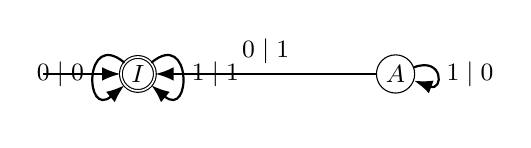
\begin{tikzpicture}[node distance=28mm]
\node[basevtx] (I) {$I$};
\node[vtx, right=of I] (A) {$A$};
\draw[edge] ($(I)+(-1.2,0)$) -- (I);

\draw[edge] (I) to[out=140,in=220,looseness=6] node[left] {$0\mid 0$} (I);
\draw[edge] (I) to[out=40,in=-40,looseness=6] node[right] {$1\mid 1$} (I);

\draw[edge] (A) -- node[above] {$0\mid 1$} (I);
\draw[edge] (A) to[out=20,in=340,looseness=6] node[right] {$1\mid 0$} (A);
\end{tikzpicture}
\caption{Binary adding machine: $A$ adds $1$ (least significant digit first, i.e.\ acting on the rooted binary tree).}
\end{figure}

\paragraph{Forward construction (Algorithm A) in one check.}
Applying $A$ to a word $w\in\{0,1\}^*$ toggles leading $1$'s to $0$ until the first $0$ becomes $1$ (carry mechanism),
which is exactly adding one in binary on each finite level $\Sigma^n$.

\paragraph{Inverse reconstruction (Algorithm B) from wreath recursion.}
State $A$ has first-letter permutation $(0\ 1)$ and sections $(A|_0,A|_1)=(I,A)$, hence
\[
A \equiv (I,A)\,(0\ 1),
\qquad
I \equiv (I,I)\,\mathrm{id},
\]
which yields $\lambda,\delta$ as above.


% \nocite{*}
\bibliographystyle{abbrv}
\bibliography{reference}



\end{document}